% ============================================================
%  TizZで描いた経済学の図をBeamerで表示するためのサンプルコード
%
%  コンパイル方法:
%    upLaTeX
% ============================================================
\documentclass[
  %aspectratio=169,       % 16:9（4:3にするなら削除）
  dvipdfmx,               % 日本語対応
  t,                      % コンテンツを上寄せ
  10pt
]{beamer}

% ── 日本語フォント（\documentclass 直後・\input より前に置く） ──
\usepackage[deluxe]{otf}           % 多ウェイト和文フォント
\usepackage[haranoaji]{pxchfon}    % ヒラギノ ProN（macOS）
% 他環境の場合は pxchfon のオプションを切り替える:
%   \usepackage[yu-osx]{pxchfon}       % 游書体（macOS）
%   \usepackage[ipaex]{pxchfon}        % IPAex（環境非依存）

% ============================================================
%  my_preamble.sty
%  upLaTeX + dvipdfmx + Beamer 用プリアンブル
%
%  使い方（\documentclass の直後に）:
%    % ============================================================
%  my_preamble.sty
%  upLaTeX + dvipdfmx + Beamer 用プリアンブル
%
%  使い方（\documentclass の直後に）:
%    % ============================================================
%  my_preamble.sty
%  upLaTeX + dvipdfmx + Beamer 用プリアンブル
%
%  使い方（\documentclass の直後に）:
%    \input{my_preamble}
%
%  前提: \documentclass[dvipdfmx, ...]{beamer}
% ============================================================

% === 数学・記号 ==============================================
% amsmath / amsfonts は Beamer が内部でロード済みなので不要
% amssymb のみ Beamer が読まないため明示的にロードする
\usepackage{amssymb}

% === 図版・作図 ==============================================
% standalone: \input で standalone クラスのファイルを取り込む際に
%   プリアンブル（\documentclass 〜 \begin{document}）を自動的に無視し、
%   本文（TikZ コード等）だけを展開する。
%   → 各 TikZ ファイルを単体コンパイルしながら Beamer にも \input できる。
\usepackage{standalone}

\usepackage{tikz}
\usetikzlibrary{arrows.meta}               % Stealth 矢印等
\usetikzlibrary{decorations.pathreplacing} % 波括弧（DiD図等）
\usetikzlibrary{shapes.geometric, positioning}          % 楕円ノード等（因果推論図）

% PGFPlots: 関数プロット・データ可視化
\usepackage{pgfplots}
\pgfplotsset{compat=1.18}
\usepgfplotslibrary{groupplots}       % 複数パネル（上下・左右配置）
\usepgfplotslibrary{fillbetween}      % 2曲線間の塗りつぶし

% === TikZ 図共通カラー ========================================
% standalone プリアンブルは \input 時に無視されるため、
% 各 TikZ ファイルで使う色はここで定義する。
\definecolor{cfcol}  {RGB}{232, 232, 232}     % 観測不可（薄灰）
\definecolor{cfgray}  {RGB}{100, 140, 200}    % 反事実（薄い青）
\definecolor{expgreen} {RGB}{200, 230, 200}   % 拡張局面シェード
\definecolor{fillcol}{RGB}{180, 215, 255}     % 政策効果の差分領域
\definecolor{gdpblue}  {RGB}{30,  90,  180}   % GDP 線・AD 曲線
\definecolor{goldcol}  {RGB}{190, 140,  10}
\definecolor{recred}   {RGB}{240, 200, 200}   % 後退局面シェード
\definecolor{srasgreen}{RGB}{30,  140, 60}    % SRAS（短期総供給曲線）
\definecolor{trendred} {RGB}{190, 40,  40}    % トレンド線・LRAS
\definecolor{obscol} {RGB}{210, 228, 255}     % 観測可能（薄青）
\definecolor{watercol}{RGB}{175, 210, 240}

% graphicx は Beamer が内部でロードするため不要
% subfigure は非推奨（TeX Live が警告を出す）。
\usepackage{subfigure}

% === 参考文献 ================================================
\usepackage{natbib}

% === 欧文フォント =============================================
% newpxtext: Palatino 改良版の本文フォント（mathpazo の現代的後継）
% newpxmath: Palatino 系数式フォント（記号セットが mathpazo より充実）
% \usefonttheme{serif} と組み合わせて Beamer 全体をセリフ体に統一
%
% 代替: Times 系にする場合は以下に切り替え
%   \usepackage{newtxtext}
%   \usepackage{newtxmath}
\usepackage{newpxtext}
\usepackage{newpxmath}

% === 日本語 ==================================================
% otf / pxchfon は \documentclass 直後のメインファイルに記述する想定
% （Beamer のクラスオプション dvipdfmx より先に読まれる必要があるため）
%
%   メインファイルの例:
%     \documentclass[dvipdfmx, t, 10pt]{beamer}
%     \usepackage[deluxe]{otf}
%     \usepackage[hiragino-pron]{pxchfon}
%     \input{my_preamble}

% hyperref の日本語対応（dvipdfmx 環境でのしおり文字化け防止）
\usepackage{pxjahyper}

% === フォントテーマ ==========================================
% 和文: \kanjifamilydefault を \gtdefault にしているのでゴシック体
% 欧文: \usefonttheme{serif} で Palatino（mathpazo）
% → 和文ゴシック + 欧文セリフ の組み合わせ（プレゼン標準）
% 和文も明朝にしたい場合は \gtdefault を \mcdefault に変更する
\renewcommand{\kanjifamilydefault}{\gtdefault}
\usefonttheme{serif}

% 行間（1.0 = デフォルト、1.1〜1.2 が「少し広め」の目安）
\linespread{1.15}

% upLaTeX のゴシック体には b（bold）ウェイトが未定義で、
% \bfseries 使用時に警告が出る。b → bx へのマッピングを明示的に
% 宣言することで警告を抑制する（JY2: 横組み、JT2: 縦組み）
\DeclareFontShape{JY2}{hgt}{b}{n}{<->ssub*hgt/bx/n}{}
\DeclareFontShape{JT2}{hgt}{b}{n}{<->ssub*hgt/bx/n}{}

% === Beamer テーマ ===========================================
\usetheme{default}
\usecolortheme{default}

% ナビゲーションバーを削除
\setbeamertemplate{navigation symbols}{}

% === カラー（モノクロ） =======================================
\setbeamercolor{normal text}{fg=black, bg=white}
\setbeamercolor{headline}{fg=black, bg=white}
\setbeamercolor{footline}{fg=black, bg=white}
\setbeamercolor{frametitle}{fg=black, bg=white}
\setbeamercolor{block title}{fg=black, bg=white}
\setbeamercolor{block body}{fg=black, bg=white}
\setbeamercolor{itemize item}{fg=black}
\setbeamercolor{itemize subitem}{fg=black}
\setbeamercolor{itemize subsubitem}{fg=black}
\setbeamercolor{enumerate item}{fg=black}
\setbeamercolor{enumerate subitem}{fg=black}
\setbeamercolor{enumerate subsubitem}{fg=black}
\setbeamercolor{alerted text}{fg=black}

% ブロックの枠をなくす
\setbeamertemplate{blocks}[default]

% === 余白 ====================================================
\setbeamersize{text margin left=5mm, text margin right=5mm}

% === メタデータ（各ファイルで上書き可） ======================
\newcommand{\coursename}{TikZ：経済学でよく使う図}
\author[山田 知明]{山田 知明}
\title{TikZ：経済学でよく使う図}
\institute[明治大学]{明治大学 商学部}
\date{2026年4月7日}

% === ヘッダー（奇数: 左上に講義名 / 偶数: 右上に講義者名） ==
% leftskip/rightskip でマージンを beamercolorbox 内に閉じ込める
\setbeamertemplate{headline}{%
  \begin{beamercolorbox}[%
    wd=\paperwidth, ht=4mm, dp=1.5mm,
    leftskip=5mm, rightskip=5mm]{headline}%
    \ifodd\insertframenumber
      {\footnotesize\coursename}\hfill
    \else
      \hfill
      {\footnotesize\insertshortauthor%
        \ifx\insertshortinstitute\@empty\else
          \ (\insertshortinstitute)%
        \fi}%
    \fi
  \end{beamercolorbox}%
  % 線：テキスト領域幅（左右 5mm マージン分を差し引く）
  \hbox{\hspace{5mm}\rule{\dimexpr\paperwidth-10mm\relax}{0.1pt}}%
}

% === フッター（右下にページ番号） ============================
% [plain] フレーム（タイトルページ等）では自動的に非表示になる
\setbeamertemplate{footline}{%
  \hbox{\hspace{5mm}\rule{\dimexpr\paperwidth-10mm\relax}{0.1pt}}%
  \begin{beamercolorbox}[%
    wd=\paperwidth, ht=2.5mm, dp=1.5mm,
    leftskip=5mm, rightskip=5mm]{footline}%
    %\hfill{\footnotesize\insertframenumber}%
    \hfill{{\footnotesize\insertframenumber\,/\,\inserttotalframenumber}}
  \end{beamercolorbox}%
}

% === フレームタイトル =========================================
\setbeamertemplate{frametitle}{%
  \vspace{1mm}%
  {\large\bfseries\insertframetitle}%
  \ifx\insertframesubtitle\@empty\else
    \\[0.5mm]{\small\itshape\insertframesubtitle}%
  \fi
  \vspace{-1mm}%
}

% === 箇条書き記号 =============================================
\setbeamertemplate{itemize item}{$\bullet$}
\setbeamertemplate{itemize subitem}{$\circ$}
\setbeamertemplate{itemize subsubitem}{--}

% === タイトルページ ===========================================
\setbeamertemplate{title page}{%
  \vfill
  \centering
  {\LARGE\bfseries\inserttitle}\\[5mm]
  {\normalsize\insertauthor}\\[2mm]
  {\normalsize\insertinstitute}\\[1mm]
  {\normalsize\insertdate}%
  \vfill
}

% === 参考文献スタイル =========================================
\bibliographystyle{ecta}

%
%  前提: \documentclass[dvipdfmx, ...]{beamer}
% ============================================================

% === 数学・記号 ==============================================
% amsmath / amsfonts は Beamer が内部でロード済みなので不要
% amssymb のみ Beamer が読まないため明示的にロードする
\usepackage{amssymb}

% === 図版・作図 ==============================================
% standalone: \input で standalone クラスのファイルを取り込む際に
%   プリアンブル（\documentclass 〜 \begin{document}）を自動的に無視し、
%   本文（TikZ コード等）だけを展開する。
%   → 各 TikZ ファイルを単体コンパイルしながら Beamer にも \input できる。
\usepackage{standalone}

\usepackage{tikz}
\usetikzlibrary{arrows.meta}               % Stealth 矢印等
\usetikzlibrary{decorations.pathreplacing} % 波括弧（DiD図等）
\usetikzlibrary{shapes.geometric, positioning}          % 楕円ノード等（因果推論図）

% PGFPlots: 関数プロット・データ可視化
\usepackage{pgfplots}
\pgfplotsset{compat=1.18}
\usepgfplotslibrary{groupplots}       % 複数パネル（上下・左右配置）
\usepgfplotslibrary{fillbetween}      % 2曲線間の塗りつぶし

% === TikZ 図共通カラー ========================================
% standalone プリアンブルは \input 時に無視されるため、
% 各 TikZ ファイルで使う色はここで定義する。
\definecolor{cfcol}  {RGB}{232, 232, 232}     % 観測不可（薄灰）
\definecolor{cfgray}  {RGB}{100, 140, 200}    % 反事実（薄い青）
\definecolor{expgreen} {RGB}{200, 230, 200}   % 拡張局面シェード
\definecolor{fillcol}{RGB}{180, 215, 255}     % 政策効果の差分領域
\definecolor{gdpblue}  {RGB}{30,  90,  180}   % GDP 線・AD 曲線
\definecolor{goldcol}  {RGB}{190, 140,  10}
\definecolor{recred}   {RGB}{240, 200, 200}   % 後退局面シェード
\definecolor{srasgreen}{RGB}{30,  140, 60}    % SRAS（短期総供給曲線）
\definecolor{trendred} {RGB}{190, 40,  40}    % トレンド線・LRAS
\definecolor{obscol} {RGB}{210, 228, 255}     % 観測可能（薄青）
\definecolor{watercol}{RGB}{175, 210, 240}

% graphicx は Beamer が内部でロードするため不要
% subfigure は非推奨（TeX Live が警告を出す）。
\usepackage{subfigure}

% === 参考文献 ================================================
\usepackage{natbib}

% === 欧文フォント =============================================
% newpxtext: Palatino 改良版の本文フォント（mathpazo の現代的後継）
% newpxmath: Palatino 系数式フォント（記号セットが mathpazo より充実）
% \usefonttheme{serif} と組み合わせて Beamer 全体をセリフ体に統一
%
% 代替: Times 系にする場合は以下に切り替え
%   \usepackage{newtxtext}
%   \usepackage{newtxmath}
\usepackage{newpxtext}
\usepackage{newpxmath}

% === 日本語 ==================================================
% otf / pxchfon は \documentclass 直後のメインファイルに記述する想定
% （Beamer のクラスオプション dvipdfmx より先に読まれる必要があるため）
%
%   メインファイルの例:
%     \documentclass[dvipdfmx, t, 10pt]{beamer}
%     \usepackage[deluxe]{otf}
%     \usepackage[hiragino-pron]{pxchfon}
%     % ============================================================
%  my_preamble.sty
%  upLaTeX + dvipdfmx + Beamer 用プリアンブル
%
%  使い方（\documentclass の直後に）:
%    \input{my_preamble}
%
%  前提: \documentclass[dvipdfmx, ...]{beamer}
% ============================================================

% === 数学・記号 ==============================================
% amsmath / amsfonts は Beamer が内部でロード済みなので不要
% amssymb のみ Beamer が読まないため明示的にロードする
\usepackage{amssymb}

% === 図版・作図 ==============================================
% standalone: \input で standalone クラスのファイルを取り込む際に
%   プリアンブル（\documentclass 〜 \begin{document}）を自動的に無視し、
%   本文（TikZ コード等）だけを展開する。
%   → 各 TikZ ファイルを単体コンパイルしながら Beamer にも \input できる。
\usepackage{standalone}

\usepackage{tikz}
\usetikzlibrary{arrows.meta}               % Stealth 矢印等
\usetikzlibrary{decorations.pathreplacing} % 波括弧（DiD図等）
\usetikzlibrary{shapes.geometric, positioning}          % 楕円ノード等（因果推論図）

% PGFPlots: 関数プロット・データ可視化
\usepackage{pgfplots}
\pgfplotsset{compat=1.18}
\usepgfplotslibrary{groupplots}       % 複数パネル（上下・左右配置）
\usepgfplotslibrary{fillbetween}      % 2曲線間の塗りつぶし

% === TikZ 図共通カラー ========================================
% standalone プリアンブルは \input 時に無視されるため、
% 各 TikZ ファイルで使う色はここで定義する。
\definecolor{cfcol}  {RGB}{232, 232, 232}     % 観測不可（薄灰）
\definecolor{cfgray}  {RGB}{100, 140, 200}    % 反事実（薄い青）
\definecolor{expgreen} {RGB}{200, 230, 200}   % 拡張局面シェード
\definecolor{fillcol}{RGB}{180, 215, 255}     % 政策効果の差分領域
\definecolor{gdpblue}  {RGB}{30,  90,  180}   % GDP 線・AD 曲線
\definecolor{goldcol}  {RGB}{190, 140,  10}
\definecolor{recred}   {RGB}{240, 200, 200}   % 後退局面シェード
\definecolor{srasgreen}{RGB}{30,  140, 60}    % SRAS（短期総供給曲線）
\definecolor{trendred} {RGB}{190, 40,  40}    % トレンド線・LRAS
\definecolor{obscol} {RGB}{210, 228, 255}     % 観測可能（薄青）
\definecolor{watercol}{RGB}{175, 210, 240}

% graphicx は Beamer が内部でロードするため不要
% subfigure は非推奨（TeX Live が警告を出す）。
\usepackage{subfigure}

% === 参考文献 ================================================
\usepackage{natbib}

% === 欧文フォント =============================================
% newpxtext: Palatino 改良版の本文フォント（mathpazo の現代的後継）
% newpxmath: Palatino 系数式フォント（記号セットが mathpazo より充実）
% \usefonttheme{serif} と組み合わせて Beamer 全体をセリフ体に統一
%
% 代替: Times 系にする場合は以下に切り替え
%   \usepackage{newtxtext}
%   \usepackage{newtxmath}
\usepackage{newpxtext}
\usepackage{newpxmath}

% === 日本語 ==================================================
% otf / pxchfon は \documentclass 直後のメインファイルに記述する想定
% （Beamer のクラスオプション dvipdfmx より先に読まれる必要があるため）
%
%   メインファイルの例:
%     \documentclass[dvipdfmx, t, 10pt]{beamer}
%     \usepackage[deluxe]{otf}
%     \usepackage[hiragino-pron]{pxchfon}
%     \input{my_preamble}

% hyperref の日本語対応（dvipdfmx 環境でのしおり文字化け防止）
\usepackage{pxjahyper}

% === フォントテーマ ==========================================
% 和文: \kanjifamilydefault を \gtdefault にしているのでゴシック体
% 欧文: \usefonttheme{serif} で Palatino（mathpazo）
% → 和文ゴシック + 欧文セリフ の組み合わせ（プレゼン標準）
% 和文も明朝にしたい場合は \gtdefault を \mcdefault に変更する
\renewcommand{\kanjifamilydefault}{\gtdefault}
\usefonttheme{serif}

% 行間（1.0 = デフォルト、1.1〜1.2 が「少し広め」の目安）
\linespread{1.15}

% upLaTeX のゴシック体には b（bold）ウェイトが未定義で、
% \bfseries 使用時に警告が出る。b → bx へのマッピングを明示的に
% 宣言することで警告を抑制する（JY2: 横組み、JT2: 縦組み）
\DeclareFontShape{JY2}{hgt}{b}{n}{<->ssub*hgt/bx/n}{}
\DeclareFontShape{JT2}{hgt}{b}{n}{<->ssub*hgt/bx/n}{}

% === Beamer テーマ ===========================================
\usetheme{default}
\usecolortheme{default}

% ナビゲーションバーを削除
\setbeamertemplate{navigation symbols}{}

% === カラー（モノクロ） =======================================
\setbeamercolor{normal text}{fg=black, bg=white}
\setbeamercolor{headline}{fg=black, bg=white}
\setbeamercolor{footline}{fg=black, bg=white}
\setbeamercolor{frametitle}{fg=black, bg=white}
\setbeamercolor{block title}{fg=black, bg=white}
\setbeamercolor{block body}{fg=black, bg=white}
\setbeamercolor{itemize item}{fg=black}
\setbeamercolor{itemize subitem}{fg=black}
\setbeamercolor{itemize subsubitem}{fg=black}
\setbeamercolor{enumerate item}{fg=black}
\setbeamercolor{enumerate subitem}{fg=black}
\setbeamercolor{enumerate subsubitem}{fg=black}
\setbeamercolor{alerted text}{fg=black}

% ブロックの枠をなくす
\setbeamertemplate{blocks}[default]

% === 余白 ====================================================
\setbeamersize{text margin left=5mm, text margin right=5mm}

% === メタデータ（各ファイルで上書き可） ======================
\newcommand{\coursename}{TikZ：経済学でよく使う図}
\author[山田 知明]{山田 知明}
\title{TikZ：経済学でよく使う図}
\institute[明治大学]{明治大学 商学部}
\date{2026年4月7日}

% === ヘッダー（奇数: 左上に講義名 / 偶数: 右上に講義者名） ==
% leftskip/rightskip でマージンを beamercolorbox 内に閉じ込める
\setbeamertemplate{headline}{%
  \begin{beamercolorbox}[%
    wd=\paperwidth, ht=4mm, dp=1.5mm,
    leftskip=5mm, rightskip=5mm]{headline}%
    \ifodd\insertframenumber
      {\footnotesize\coursename}\hfill
    \else
      \hfill
      {\footnotesize\insertshortauthor%
        \ifx\insertshortinstitute\@empty\else
          \ (\insertshortinstitute)%
        \fi}%
    \fi
  \end{beamercolorbox}%
  % 線：テキスト領域幅（左右 5mm マージン分を差し引く）
  \hbox{\hspace{5mm}\rule{\dimexpr\paperwidth-10mm\relax}{0.1pt}}%
}

% === フッター（右下にページ番号） ============================
% [plain] フレーム（タイトルページ等）では自動的に非表示になる
\setbeamertemplate{footline}{%
  \hbox{\hspace{5mm}\rule{\dimexpr\paperwidth-10mm\relax}{0.1pt}}%
  \begin{beamercolorbox}[%
    wd=\paperwidth, ht=2.5mm, dp=1.5mm,
    leftskip=5mm, rightskip=5mm]{footline}%
    %\hfill{\footnotesize\insertframenumber}%
    \hfill{{\footnotesize\insertframenumber\,/\,\inserttotalframenumber}}
  \end{beamercolorbox}%
}

% === フレームタイトル =========================================
\setbeamertemplate{frametitle}{%
  \vspace{1mm}%
  {\large\bfseries\insertframetitle}%
  \ifx\insertframesubtitle\@empty\else
    \\[0.5mm]{\small\itshape\insertframesubtitle}%
  \fi
  \vspace{-1mm}%
}

% === 箇条書き記号 =============================================
\setbeamertemplate{itemize item}{$\bullet$}
\setbeamertemplate{itemize subitem}{$\circ$}
\setbeamertemplate{itemize subsubitem}{--}

% === タイトルページ ===========================================
\setbeamertemplate{title page}{%
  \vfill
  \centering
  {\LARGE\bfseries\inserttitle}\\[5mm]
  {\normalsize\insertauthor}\\[2mm]
  {\normalsize\insertinstitute}\\[1mm]
  {\normalsize\insertdate}%
  \vfill
}

% === 参考文献スタイル =========================================
\bibliographystyle{ecta}


% hyperref の日本語対応（dvipdfmx 環境でのしおり文字化け防止）
\usepackage{pxjahyper}

% === フォントテーマ ==========================================
% 和文: \kanjifamilydefault を \gtdefault にしているのでゴシック体
% 欧文: \usefonttheme{serif} で Palatino（mathpazo）
% → 和文ゴシック + 欧文セリフ の組み合わせ（プレゼン標準）
% 和文も明朝にしたい場合は \gtdefault を \mcdefault に変更する
\renewcommand{\kanjifamilydefault}{\gtdefault}
\usefonttheme{serif}

% 行間（1.0 = デフォルト、1.1〜1.2 が「少し広め」の目安）
\linespread{1.15}

% upLaTeX のゴシック体には b（bold）ウェイトが未定義で、
% \bfseries 使用時に警告が出る。b → bx へのマッピングを明示的に
% 宣言することで警告を抑制する（JY2: 横組み、JT2: 縦組み）
\DeclareFontShape{JY2}{hgt}{b}{n}{<->ssub*hgt/bx/n}{}
\DeclareFontShape{JT2}{hgt}{b}{n}{<->ssub*hgt/bx/n}{}

% === Beamer テーマ ===========================================
\usetheme{default}
\usecolortheme{default}

% ナビゲーションバーを削除
\setbeamertemplate{navigation symbols}{}

% === カラー（モノクロ） =======================================
\setbeamercolor{normal text}{fg=black, bg=white}
\setbeamercolor{headline}{fg=black, bg=white}
\setbeamercolor{footline}{fg=black, bg=white}
\setbeamercolor{frametitle}{fg=black, bg=white}
\setbeamercolor{block title}{fg=black, bg=white}
\setbeamercolor{block body}{fg=black, bg=white}
\setbeamercolor{itemize item}{fg=black}
\setbeamercolor{itemize subitem}{fg=black}
\setbeamercolor{itemize subsubitem}{fg=black}
\setbeamercolor{enumerate item}{fg=black}
\setbeamercolor{enumerate subitem}{fg=black}
\setbeamercolor{enumerate subsubitem}{fg=black}
\setbeamercolor{alerted text}{fg=black}

% ブロックの枠をなくす
\setbeamertemplate{blocks}[default]

% === 余白 ====================================================
\setbeamersize{text margin left=5mm, text margin right=5mm}

% === メタデータ（各ファイルで上書き可） ======================
\newcommand{\coursename}{TikZ：経済学でよく使う図}
\author[山田 知明]{山田 知明}
\title{TikZ：経済学でよく使う図}
\institute[明治大学]{明治大学 商学部}
\date{2026年4月7日}

% === ヘッダー（奇数: 左上に講義名 / 偶数: 右上に講義者名） ==
% leftskip/rightskip でマージンを beamercolorbox 内に閉じ込める
\setbeamertemplate{headline}{%
  \begin{beamercolorbox}[%
    wd=\paperwidth, ht=4mm, dp=1.5mm,
    leftskip=5mm, rightskip=5mm]{headline}%
    \ifodd\insertframenumber
      {\footnotesize\coursename}\hfill
    \else
      \hfill
      {\footnotesize\insertshortauthor%
        \ifx\insertshortinstitute\@empty\else
          \ (\insertshortinstitute)%
        \fi}%
    \fi
  \end{beamercolorbox}%
  % 線：テキスト領域幅（左右 5mm マージン分を差し引く）
  \hbox{\hspace{5mm}\rule{\dimexpr\paperwidth-10mm\relax}{0.1pt}}%
}

% === フッター（右下にページ番号） ============================
% [plain] フレーム（タイトルページ等）では自動的に非表示になる
\setbeamertemplate{footline}{%
  \hbox{\hspace{5mm}\rule{\dimexpr\paperwidth-10mm\relax}{0.1pt}}%
  \begin{beamercolorbox}[%
    wd=\paperwidth, ht=2.5mm, dp=1.5mm,
    leftskip=5mm, rightskip=5mm]{footline}%
    %\hfill{\footnotesize\insertframenumber}%
    \hfill{{\footnotesize\insertframenumber\,/\,\inserttotalframenumber}}
  \end{beamercolorbox}%
}

% === フレームタイトル =========================================
\setbeamertemplate{frametitle}{%
  \vspace{1mm}%
  {\large\bfseries\insertframetitle}%
  \ifx\insertframesubtitle\@empty\else
    \\[0.5mm]{\small\itshape\insertframesubtitle}%
  \fi
  \vspace{-1mm}%
}

% === 箇条書き記号 =============================================
\setbeamertemplate{itemize item}{$\bullet$}
\setbeamertemplate{itemize subitem}{$\circ$}
\setbeamertemplate{itemize subsubitem}{--}

% === タイトルページ ===========================================
\setbeamertemplate{title page}{%
  \vfill
  \centering
  {\LARGE\bfseries\inserttitle}\\[5mm]
  {\normalsize\insertauthor}\\[2mm]
  {\normalsize\insertinstitute}\\[1mm]
  {\normalsize\insertdate}%
  \vfill
}

% === 参考文献スタイル =========================================
\bibliographystyle{ecta}

%
%  前提: \documentclass[dvipdfmx, ...]{beamer}
% ============================================================

% === 数学・記号 ==============================================
% amsmath / amsfonts は Beamer が内部でロード済みなので不要
% amssymb のみ Beamer が読まないため明示的にロードする
\usepackage{amssymb}

% === 図版・作図 ==============================================
% standalone: \input で standalone クラスのファイルを取り込む際に
%   プリアンブル（\documentclass 〜 \begin{document}）を自動的に無視し、
%   本文（TikZ コード等）だけを展開する。
%   → 各 TikZ ファイルを単体コンパイルしながら Beamer にも \input できる。
\usepackage{standalone}

\usepackage{tikz}
\usetikzlibrary{arrows.meta}               % Stealth 矢印等
\usetikzlibrary{decorations.pathreplacing} % 波括弧（DiD図等）
\usetikzlibrary{shapes.geometric, positioning}          % 楕円ノード等（因果推論図）

% PGFPlots: 関数プロット・データ可視化
\usepackage{pgfplots}
\pgfplotsset{compat=1.18}
\usepgfplotslibrary{groupplots}       % 複数パネル（上下・左右配置）
\usepgfplotslibrary{fillbetween}      % 2曲線間の塗りつぶし

% === TikZ 図共通カラー ========================================
% standalone プリアンブルは \input 時に無視されるため、
% 各 TikZ ファイルで使う色はここで定義する。
\definecolor{cfcol}  {RGB}{232, 232, 232}     % 観測不可（薄灰）
\definecolor{cfgray}  {RGB}{100, 140, 200}    % 反事実（薄い青）
\definecolor{expgreen} {RGB}{200, 230, 200}   % 拡張局面シェード
\definecolor{fillcol}{RGB}{180, 215, 255}     % 政策効果の差分領域
\definecolor{gdpblue}  {RGB}{30,  90,  180}   % GDP 線・AD 曲線
\definecolor{goldcol}  {RGB}{190, 140,  10}
\definecolor{recred}   {RGB}{240, 200, 200}   % 後退局面シェード
\definecolor{srasgreen}{RGB}{30,  140, 60}    % SRAS（短期総供給曲線）
\definecolor{trendred} {RGB}{190, 40,  40}    % トレンド線・LRAS
\definecolor{obscol} {RGB}{210, 228, 255}     % 観測可能（薄青）
\definecolor{watercol}{RGB}{175, 210, 240}

% graphicx は Beamer が内部でロードするため不要
% subfigure は非推奨（TeX Live が警告を出す）。
\usepackage{subfigure}

% === 参考文献 ================================================
\usepackage{natbib}

% === 欧文フォント =============================================
% newpxtext: Palatino 改良版の本文フォント（mathpazo の現代的後継）
% newpxmath: Palatino 系数式フォント（記号セットが mathpazo より充実）
% \usefonttheme{serif} と組み合わせて Beamer 全体をセリフ体に統一
%
% 代替: Times 系にする場合は以下に切り替え
%   \usepackage{newtxtext}
%   \usepackage{newtxmath}
\usepackage{newpxtext}
\usepackage{newpxmath}

% === 日本語 ==================================================
% otf / pxchfon は \documentclass 直後のメインファイルに記述する想定
% （Beamer のクラスオプション dvipdfmx より先に読まれる必要があるため）
%
%   メインファイルの例:
%     \documentclass[dvipdfmx, t, 10pt]{beamer}
%     \usepackage[deluxe]{otf}
%     \usepackage[hiragino-pron]{pxchfon}
%     % ============================================================
%  my_preamble.sty
%  upLaTeX + dvipdfmx + Beamer 用プリアンブル
%
%  使い方（\documentclass の直後に）:
%    % ============================================================
%  my_preamble.sty
%  upLaTeX + dvipdfmx + Beamer 用プリアンブル
%
%  使い方（\documentclass の直後に）:
%    \input{my_preamble}
%
%  前提: \documentclass[dvipdfmx, ...]{beamer}
% ============================================================

% === 数学・記号 ==============================================
% amsmath / amsfonts は Beamer が内部でロード済みなので不要
% amssymb のみ Beamer が読まないため明示的にロードする
\usepackage{amssymb}

% === 図版・作図 ==============================================
% standalone: \input で standalone クラスのファイルを取り込む際に
%   プリアンブル（\documentclass 〜 \begin{document}）を自動的に無視し、
%   本文（TikZ コード等）だけを展開する。
%   → 各 TikZ ファイルを単体コンパイルしながら Beamer にも \input できる。
\usepackage{standalone}

\usepackage{tikz}
\usetikzlibrary{arrows.meta}               % Stealth 矢印等
\usetikzlibrary{decorations.pathreplacing} % 波括弧（DiD図等）
\usetikzlibrary{shapes.geometric, positioning}          % 楕円ノード等（因果推論図）

% PGFPlots: 関数プロット・データ可視化
\usepackage{pgfplots}
\pgfplotsset{compat=1.18}
\usepgfplotslibrary{groupplots}       % 複数パネル（上下・左右配置）
\usepgfplotslibrary{fillbetween}      % 2曲線間の塗りつぶし

% === TikZ 図共通カラー ========================================
% standalone プリアンブルは \input 時に無視されるため、
% 各 TikZ ファイルで使う色はここで定義する。
\definecolor{cfcol}  {RGB}{232, 232, 232}     % 観測不可（薄灰）
\definecolor{cfgray}  {RGB}{100, 140, 200}    % 反事実（薄い青）
\definecolor{expgreen} {RGB}{200, 230, 200}   % 拡張局面シェード
\definecolor{fillcol}{RGB}{180, 215, 255}     % 政策効果の差分領域
\definecolor{gdpblue}  {RGB}{30,  90,  180}   % GDP 線・AD 曲線
\definecolor{goldcol}  {RGB}{190, 140,  10}
\definecolor{recred}   {RGB}{240, 200, 200}   % 後退局面シェード
\definecolor{srasgreen}{RGB}{30,  140, 60}    % SRAS（短期総供給曲線）
\definecolor{trendred} {RGB}{190, 40,  40}    % トレンド線・LRAS
\definecolor{obscol} {RGB}{210, 228, 255}     % 観測可能（薄青）
\definecolor{watercol}{RGB}{175, 210, 240}

% graphicx は Beamer が内部でロードするため不要
% subfigure は非推奨（TeX Live が警告を出す）。
\usepackage{subfigure}

% === 参考文献 ================================================
\usepackage{natbib}

% === 欧文フォント =============================================
% newpxtext: Palatino 改良版の本文フォント（mathpazo の現代的後継）
% newpxmath: Palatino 系数式フォント（記号セットが mathpazo より充実）
% \usefonttheme{serif} と組み合わせて Beamer 全体をセリフ体に統一
%
% 代替: Times 系にする場合は以下に切り替え
%   \usepackage{newtxtext}
%   \usepackage{newtxmath}
\usepackage{newpxtext}
\usepackage{newpxmath}

% === 日本語 ==================================================
% otf / pxchfon は \documentclass 直後のメインファイルに記述する想定
% （Beamer のクラスオプション dvipdfmx より先に読まれる必要があるため）
%
%   メインファイルの例:
%     \documentclass[dvipdfmx, t, 10pt]{beamer}
%     \usepackage[deluxe]{otf}
%     \usepackage[hiragino-pron]{pxchfon}
%     \input{my_preamble}

% hyperref の日本語対応（dvipdfmx 環境でのしおり文字化け防止）
\usepackage{pxjahyper}

% === フォントテーマ ==========================================
% 和文: \kanjifamilydefault を \gtdefault にしているのでゴシック体
% 欧文: \usefonttheme{serif} で Palatino（mathpazo）
% → 和文ゴシック + 欧文セリフ の組み合わせ（プレゼン標準）
% 和文も明朝にしたい場合は \gtdefault を \mcdefault に変更する
\renewcommand{\kanjifamilydefault}{\gtdefault}
\usefonttheme{serif}

% 行間（1.0 = デフォルト、1.1〜1.2 が「少し広め」の目安）
\linespread{1.15}

% upLaTeX のゴシック体には b（bold）ウェイトが未定義で、
% \bfseries 使用時に警告が出る。b → bx へのマッピングを明示的に
% 宣言することで警告を抑制する（JY2: 横組み、JT2: 縦組み）
\DeclareFontShape{JY2}{hgt}{b}{n}{<->ssub*hgt/bx/n}{}
\DeclareFontShape{JT2}{hgt}{b}{n}{<->ssub*hgt/bx/n}{}

% === Beamer テーマ ===========================================
\usetheme{default}
\usecolortheme{default}

% ナビゲーションバーを削除
\setbeamertemplate{navigation symbols}{}

% === カラー（モノクロ） =======================================
\setbeamercolor{normal text}{fg=black, bg=white}
\setbeamercolor{headline}{fg=black, bg=white}
\setbeamercolor{footline}{fg=black, bg=white}
\setbeamercolor{frametitle}{fg=black, bg=white}
\setbeamercolor{block title}{fg=black, bg=white}
\setbeamercolor{block body}{fg=black, bg=white}
\setbeamercolor{itemize item}{fg=black}
\setbeamercolor{itemize subitem}{fg=black}
\setbeamercolor{itemize subsubitem}{fg=black}
\setbeamercolor{enumerate item}{fg=black}
\setbeamercolor{enumerate subitem}{fg=black}
\setbeamercolor{enumerate subsubitem}{fg=black}
\setbeamercolor{alerted text}{fg=black}

% ブロックの枠をなくす
\setbeamertemplate{blocks}[default]

% === 余白 ====================================================
\setbeamersize{text margin left=5mm, text margin right=5mm}

% === メタデータ（各ファイルで上書き可） ======================
\newcommand{\coursename}{TikZ：経済学でよく使う図}
\author[山田 知明]{山田 知明}
\title{TikZ：経済学でよく使う図}
\institute[明治大学]{明治大学 商学部}
\date{2026年4月7日}

% === ヘッダー（奇数: 左上に講義名 / 偶数: 右上に講義者名） ==
% leftskip/rightskip でマージンを beamercolorbox 内に閉じ込める
\setbeamertemplate{headline}{%
  \begin{beamercolorbox}[%
    wd=\paperwidth, ht=4mm, dp=1.5mm,
    leftskip=5mm, rightskip=5mm]{headline}%
    \ifodd\insertframenumber
      {\footnotesize\coursename}\hfill
    \else
      \hfill
      {\footnotesize\insertshortauthor%
        \ifx\insertshortinstitute\@empty\else
          \ (\insertshortinstitute)%
        \fi}%
    \fi
  \end{beamercolorbox}%
  % 線：テキスト領域幅（左右 5mm マージン分を差し引く）
  \hbox{\hspace{5mm}\rule{\dimexpr\paperwidth-10mm\relax}{0.1pt}}%
}

% === フッター（右下にページ番号） ============================
% [plain] フレーム（タイトルページ等）では自動的に非表示になる
\setbeamertemplate{footline}{%
  \hbox{\hspace{5mm}\rule{\dimexpr\paperwidth-10mm\relax}{0.1pt}}%
  \begin{beamercolorbox}[%
    wd=\paperwidth, ht=2.5mm, dp=1.5mm,
    leftskip=5mm, rightskip=5mm]{footline}%
    %\hfill{\footnotesize\insertframenumber}%
    \hfill{{\footnotesize\insertframenumber\,/\,\inserttotalframenumber}}
  \end{beamercolorbox}%
}

% === フレームタイトル =========================================
\setbeamertemplate{frametitle}{%
  \vspace{1mm}%
  {\large\bfseries\insertframetitle}%
  \ifx\insertframesubtitle\@empty\else
    \\[0.5mm]{\small\itshape\insertframesubtitle}%
  \fi
  \vspace{-1mm}%
}

% === 箇条書き記号 =============================================
\setbeamertemplate{itemize item}{$\bullet$}
\setbeamertemplate{itemize subitem}{$\circ$}
\setbeamertemplate{itemize subsubitem}{--}

% === タイトルページ ===========================================
\setbeamertemplate{title page}{%
  \vfill
  \centering
  {\LARGE\bfseries\inserttitle}\\[5mm]
  {\normalsize\insertauthor}\\[2mm]
  {\normalsize\insertinstitute}\\[1mm]
  {\normalsize\insertdate}%
  \vfill
}

% === 参考文献スタイル =========================================
\bibliographystyle{ecta}

%
%  前提: \documentclass[dvipdfmx, ...]{beamer}
% ============================================================

% === 数学・記号 ==============================================
% amsmath / amsfonts は Beamer が内部でロード済みなので不要
% amssymb のみ Beamer が読まないため明示的にロードする
\usepackage{amssymb}

% === 図版・作図 ==============================================
% standalone: \input で standalone クラスのファイルを取り込む際に
%   プリアンブル（\documentclass 〜 \begin{document}）を自動的に無視し、
%   本文（TikZ コード等）だけを展開する。
%   → 各 TikZ ファイルを単体コンパイルしながら Beamer にも \input できる。
\usepackage{standalone}

\usepackage{tikz}
\usetikzlibrary{arrows.meta}               % Stealth 矢印等
\usetikzlibrary{decorations.pathreplacing} % 波括弧（DiD図等）
\usetikzlibrary{shapes.geometric, positioning}          % 楕円ノード等（因果推論図）

% PGFPlots: 関数プロット・データ可視化
\usepackage{pgfplots}
\pgfplotsset{compat=1.18}
\usepgfplotslibrary{groupplots}       % 複数パネル（上下・左右配置）
\usepgfplotslibrary{fillbetween}      % 2曲線間の塗りつぶし

% === TikZ 図共通カラー ========================================
% standalone プリアンブルは \input 時に無視されるため、
% 各 TikZ ファイルで使う色はここで定義する。
\definecolor{cfcol}  {RGB}{232, 232, 232}     % 観測不可（薄灰）
\definecolor{cfgray}  {RGB}{100, 140, 200}    % 反事実（薄い青）
\definecolor{expgreen} {RGB}{200, 230, 200}   % 拡張局面シェード
\definecolor{fillcol}{RGB}{180, 215, 255}     % 政策効果の差分領域
\definecolor{gdpblue}  {RGB}{30,  90,  180}   % GDP 線・AD 曲線
\definecolor{goldcol}  {RGB}{190, 140,  10}
\definecolor{recred}   {RGB}{240, 200, 200}   % 後退局面シェード
\definecolor{srasgreen}{RGB}{30,  140, 60}    % SRAS（短期総供給曲線）
\definecolor{trendred} {RGB}{190, 40,  40}    % トレンド線・LRAS
\definecolor{obscol} {RGB}{210, 228, 255}     % 観測可能（薄青）
\definecolor{watercol}{RGB}{175, 210, 240}

% graphicx は Beamer が内部でロードするため不要
% subfigure は非推奨（TeX Live が警告を出す）。
\usepackage{subfigure}

% === 参考文献 ================================================
\usepackage{natbib}

% === 欧文フォント =============================================
% newpxtext: Palatino 改良版の本文フォント（mathpazo の現代的後継）
% newpxmath: Palatino 系数式フォント（記号セットが mathpazo より充実）
% \usefonttheme{serif} と組み合わせて Beamer 全体をセリフ体に統一
%
% 代替: Times 系にする場合は以下に切り替え
%   \usepackage{newtxtext}
%   \usepackage{newtxmath}
\usepackage{newpxtext}
\usepackage{newpxmath}

% === 日本語 ==================================================
% otf / pxchfon は \documentclass 直後のメインファイルに記述する想定
% （Beamer のクラスオプション dvipdfmx より先に読まれる必要があるため）
%
%   メインファイルの例:
%     \documentclass[dvipdfmx, t, 10pt]{beamer}
%     \usepackage[deluxe]{otf}
%     \usepackage[hiragino-pron]{pxchfon}
%     % ============================================================
%  my_preamble.sty
%  upLaTeX + dvipdfmx + Beamer 用プリアンブル
%
%  使い方（\documentclass の直後に）:
%    \input{my_preamble}
%
%  前提: \documentclass[dvipdfmx, ...]{beamer}
% ============================================================

% === 数学・記号 ==============================================
% amsmath / amsfonts は Beamer が内部でロード済みなので不要
% amssymb のみ Beamer が読まないため明示的にロードする
\usepackage{amssymb}

% === 図版・作図 ==============================================
% standalone: \input で standalone クラスのファイルを取り込む際に
%   プリアンブル（\documentclass 〜 \begin{document}）を自動的に無視し、
%   本文（TikZ コード等）だけを展開する。
%   → 各 TikZ ファイルを単体コンパイルしながら Beamer にも \input できる。
\usepackage{standalone}

\usepackage{tikz}
\usetikzlibrary{arrows.meta}               % Stealth 矢印等
\usetikzlibrary{decorations.pathreplacing} % 波括弧（DiD図等）
\usetikzlibrary{shapes.geometric, positioning}          % 楕円ノード等（因果推論図）

% PGFPlots: 関数プロット・データ可視化
\usepackage{pgfplots}
\pgfplotsset{compat=1.18}
\usepgfplotslibrary{groupplots}       % 複数パネル（上下・左右配置）
\usepgfplotslibrary{fillbetween}      % 2曲線間の塗りつぶし

% === TikZ 図共通カラー ========================================
% standalone プリアンブルは \input 時に無視されるため、
% 各 TikZ ファイルで使う色はここで定義する。
\definecolor{cfcol}  {RGB}{232, 232, 232}     % 観測不可（薄灰）
\definecolor{cfgray}  {RGB}{100, 140, 200}    % 反事実（薄い青）
\definecolor{expgreen} {RGB}{200, 230, 200}   % 拡張局面シェード
\definecolor{fillcol}{RGB}{180, 215, 255}     % 政策効果の差分領域
\definecolor{gdpblue}  {RGB}{30,  90,  180}   % GDP 線・AD 曲線
\definecolor{goldcol}  {RGB}{190, 140,  10}
\definecolor{recred}   {RGB}{240, 200, 200}   % 後退局面シェード
\definecolor{srasgreen}{RGB}{30,  140, 60}    % SRAS（短期総供給曲線）
\definecolor{trendred} {RGB}{190, 40,  40}    % トレンド線・LRAS
\definecolor{obscol} {RGB}{210, 228, 255}     % 観測可能（薄青）
\definecolor{watercol}{RGB}{175, 210, 240}

% graphicx は Beamer が内部でロードするため不要
% subfigure は非推奨（TeX Live が警告を出す）。
\usepackage{subfigure}

% === 参考文献 ================================================
\usepackage{natbib}

% === 欧文フォント =============================================
% newpxtext: Palatino 改良版の本文フォント（mathpazo の現代的後継）
% newpxmath: Palatino 系数式フォント（記号セットが mathpazo より充実）
% \usefonttheme{serif} と組み合わせて Beamer 全体をセリフ体に統一
%
% 代替: Times 系にする場合は以下に切り替え
%   \usepackage{newtxtext}
%   \usepackage{newtxmath}
\usepackage{newpxtext}
\usepackage{newpxmath}

% === 日本語 ==================================================
% otf / pxchfon は \documentclass 直後のメインファイルに記述する想定
% （Beamer のクラスオプション dvipdfmx より先に読まれる必要があるため）
%
%   メインファイルの例:
%     \documentclass[dvipdfmx, t, 10pt]{beamer}
%     \usepackage[deluxe]{otf}
%     \usepackage[hiragino-pron]{pxchfon}
%     \input{my_preamble}

% hyperref の日本語対応（dvipdfmx 環境でのしおり文字化け防止）
\usepackage{pxjahyper}

% === フォントテーマ ==========================================
% 和文: \kanjifamilydefault を \gtdefault にしているのでゴシック体
% 欧文: \usefonttheme{serif} で Palatino（mathpazo）
% → 和文ゴシック + 欧文セリフ の組み合わせ（プレゼン標準）
% 和文も明朝にしたい場合は \gtdefault を \mcdefault に変更する
\renewcommand{\kanjifamilydefault}{\gtdefault}
\usefonttheme{serif}

% 行間（1.0 = デフォルト、1.1〜1.2 が「少し広め」の目安）
\linespread{1.15}

% upLaTeX のゴシック体には b（bold）ウェイトが未定義で、
% \bfseries 使用時に警告が出る。b → bx へのマッピングを明示的に
% 宣言することで警告を抑制する（JY2: 横組み、JT2: 縦組み）
\DeclareFontShape{JY2}{hgt}{b}{n}{<->ssub*hgt/bx/n}{}
\DeclareFontShape{JT2}{hgt}{b}{n}{<->ssub*hgt/bx/n}{}

% === Beamer テーマ ===========================================
\usetheme{default}
\usecolortheme{default}

% ナビゲーションバーを削除
\setbeamertemplate{navigation symbols}{}

% === カラー（モノクロ） =======================================
\setbeamercolor{normal text}{fg=black, bg=white}
\setbeamercolor{headline}{fg=black, bg=white}
\setbeamercolor{footline}{fg=black, bg=white}
\setbeamercolor{frametitle}{fg=black, bg=white}
\setbeamercolor{block title}{fg=black, bg=white}
\setbeamercolor{block body}{fg=black, bg=white}
\setbeamercolor{itemize item}{fg=black}
\setbeamercolor{itemize subitem}{fg=black}
\setbeamercolor{itemize subsubitem}{fg=black}
\setbeamercolor{enumerate item}{fg=black}
\setbeamercolor{enumerate subitem}{fg=black}
\setbeamercolor{enumerate subsubitem}{fg=black}
\setbeamercolor{alerted text}{fg=black}

% ブロックの枠をなくす
\setbeamertemplate{blocks}[default]

% === 余白 ====================================================
\setbeamersize{text margin left=5mm, text margin right=5mm}

% === メタデータ（各ファイルで上書き可） ======================
\newcommand{\coursename}{TikZ：経済学でよく使う図}
\author[山田 知明]{山田 知明}
\title{TikZ：経済学でよく使う図}
\institute[明治大学]{明治大学 商学部}
\date{2026年4月7日}

% === ヘッダー（奇数: 左上に講義名 / 偶数: 右上に講義者名） ==
% leftskip/rightskip でマージンを beamercolorbox 内に閉じ込める
\setbeamertemplate{headline}{%
  \begin{beamercolorbox}[%
    wd=\paperwidth, ht=4mm, dp=1.5mm,
    leftskip=5mm, rightskip=5mm]{headline}%
    \ifodd\insertframenumber
      {\footnotesize\coursename}\hfill
    \else
      \hfill
      {\footnotesize\insertshortauthor%
        \ifx\insertshortinstitute\@empty\else
          \ (\insertshortinstitute)%
        \fi}%
    \fi
  \end{beamercolorbox}%
  % 線：テキスト領域幅（左右 5mm マージン分を差し引く）
  \hbox{\hspace{5mm}\rule{\dimexpr\paperwidth-10mm\relax}{0.1pt}}%
}

% === フッター（右下にページ番号） ============================
% [plain] フレーム（タイトルページ等）では自動的に非表示になる
\setbeamertemplate{footline}{%
  \hbox{\hspace{5mm}\rule{\dimexpr\paperwidth-10mm\relax}{0.1pt}}%
  \begin{beamercolorbox}[%
    wd=\paperwidth, ht=2.5mm, dp=1.5mm,
    leftskip=5mm, rightskip=5mm]{footline}%
    %\hfill{\footnotesize\insertframenumber}%
    \hfill{{\footnotesize\insertframenumber\,/\,\inserttotalframenumber}}
  \end{beamercolorbox}%
}

% === フレームタイトル =========================================
\setbeamertemplate{frametitle}{%
  \vspace{1mm}%
  {\large\bfseries\insertframetitle}%
  \ifx\insertframesubtitle\@empty\else
    \\[0.5mm]{\small\itshape\insertframesubtitle}%
  \fi
  \vspace{-1mm}%
}

% === 箇条書き記号 =============================================
\setbeamertemplate{itemize item}{$\bullet$}
\setbeamertemplate{itemize subitem}{$\circ$}
\setbeamertemplate{itemize subsubitem}{--}

% === タイトルページ ===========================================
\setbeamertemplate{title page}{%
  \vfill
  \centering
  {\LARGE\bfseries\inserttitle}\\[5mm]
  {\normalsize\insertauthor}\\[2mm]
  {\normalsize\insertinstitute}\\[1mm]
  {\normalsize\insertdate}%
  \vfill
}

% === 参考文献スタイル =========================================
\bibliographystyle{ecta}


% hyperref の日本語対応（dvipdfmx 環境でのしおり文字化け防止）
\usepackage{pxjahyper}

% === フォントテーマ ==========================================
% 和文: \kanjifamilydefault を \gtdefault にしているのでゴシック体
% 欧文: \usefonttheme{serif} で Palatino（mathpazo）
% → 和文ゴシック + 欧文セリフ の組み合わせ（プレゼン標準）
% 和文も明朝にしたい場合は \gtdefault を \mcdefault に変更する
\renewcommand{\kanjifamilydefault}{\gtdefault}
\usefonttheme{serif}

% 行間（1.0 = デフォルト、1.1〜1.2 が「少し広め」の目安）
\linespread{1.15}

% upLaTeX のゴシック体には b（bold）ウェイトが未定義で、
% \bfseries 使用時に警告が出る。b → bx へのマッピングを明示的に
% 宣言することで警告を抑制する（JY2: 横組み、JT2: 縦組み）
\DeclareFontShape{JY2}{hgt}{b}{n}{<->ssub*hgt/bx/n}{}
\DeclareFontShape{JT2}{hgt}{b}{n}{<->ssub*hgt/bx/n}{}

% === Beamer テーマ ===========================================
\usetheme{default}
\usecolortheme{default}

% ナビゲーションバーを削除
\setbeamertemplate{navigation symbols}{}

% === カラー（モノクロ） =======================================
\setbeamercolor{normal text}{fg=black, bg=white}
\setbeamercolor{headline}{fg=black, bg=white}
\setbeamercolor{footline}{fg=black, bg=white}
\setbeamercolor{frametitle}{fg=black, bg=white}
\setbeamercolor{block title}{fg=black, bg=white}
\setbeamercolor{block body}{fg=black, bg=white}
\setbeamercolor{itemize item}{fg=black}
\setbeamercolor{itemize subitem}{fg=black}
\setbeamercolor{itemize subsubitem}{fg=black}
\setbeamercolor{enumerate item}{fg=black}
\setbeamercolor{enumerate subitem}{fg=black}
\setbeamercolor{enumerate subsubitem}{fg=black}
\setbeamercolor{alerted text}{fg=black}

% ブロックの枠をなくす
\setbeamertemplate{blocks}[default]

% === 余白 ====================================================
\setbeamersize{text margin left=5mm, text margin right=5mm}

% === メタデータ（各ファイルで上書き可） ======================
\newcommand{\coursename}{TikZ：経済学でよく使う図}
\author[山田 知明]{山田 知明}
\title{TikZ：経済学でよく使う図}
\institute[明治大学]{明治大学 商学部}
\date{2026年4月7日}

% === ヘッダー（奇数: 左上に講義名 / 偶数: 右上に講義者名） ==
% leftskip/rightskip でマージンを beamercolorbox 内に閉じ込める
\setbeamertemplate{headline}{%
  \begin{beamercolorbox}[%
    wd=\paperwidth, ht=4mm, dp=1.5mm,
    leftskip=5mm, rightskip=5mm]{headline}%
    \ifodd\insertframenumber
      {\footnotesize\coursename}\hfill
    \else
      \hfill
      {\footnotesize\insertshortauthor%
        \ifx\insertshortinstitute\@empty\else
          \ (\insertshortinstitute)%
        \fi}%
    \fi
  \end{beamercolorbox}%
  % 線：テキスト領域幅（左右 5mm マージン分を差し引く）
  \hbox{\hspace{5mm}\rule{\dimexpr\paperwidth-10mm\relax}{0.1pt}}%
}

% === フッター（右下にページ番号） ============================
% [plain] フレーム（タイトルページ等）では自動的に非表示になる
\setbeamertemplate{footline}{%
  \hbox{\hspace{5mm}\rule{\dimexpr\paperwidth-10mm\relax}{0.1pt}}%
  \begin{beamercolorbox}[%
    wd=\paperwidth, ht=2.5mm, dp=1.5mm,
    leftskip=5mm, rightskip=5mm]{footline}%
    %\hfill{\footnotesize\insertframenumber}%
    \hfill{{\footnotesize\insertframenumber\,/\,\inserttotalframenumber}}
  \end{beamercolorbox}%
}

% === フレームタイトル =========================================
\setbeamertemplate{frametitle}{%
  \vspace{1mm}%
  {\large\bfseries\insertframetitle}%
  \ifx\insertframesubtitle\@empty\else
    \\[0.5mm]{\small\itshape\insertframesubtitle}%
  \fi
  \vspace{-1mm}%
}

% === 箇条書き記号 =============================================
\setbeamertemplate{itemize item}{$\bullet$}
\setbeamertemplate{itemize subitem}{$\circ$}
\setbeamertemplate{itemize subsubitem}{--}

% === タイトルページ ===========================================
\setbeamertemplate{title page}{%
  \vfill
  \centering
  {\LARGE\bfseries\inserttitle}\\[5mm]
  {\normalsize\insertauthor}\\[2mm]
  {\normalsize\insertinstitute}\\[1mm]
  {\normalsize\insertdate}%
  \vfill
}

% === 参考文献スタイル =========================================
\bibliographystyle{ecta}


% hyperref の日本語対応（dvipdfmx 環境でのしおり文字化け防止）
\usepackage{pxjahyper}

% === フォントテーマ ==========================================
% 和文: \kanjifamilydefault を \gtdefault にしているのでゴシック体
% 欧文: \usefonttheme{serif} で Palatino（mathpazo）
% → 和文ゴシック + 欧文セリフ の組み合わせ（プレゼン標準）
% 和文も明朝にしたい場合は \gtdefault を \mcdefault に変更する
\renewcommand{\kanjifamilydefault}{\gtdefault}
\usefonttheme{serif}

% 行間（1.0 = デフォルト、1.1〜1.2 が「少し広め」の目安）
\linespread{1.15}

% upLaTeX のゴシック体には b（bold）ウェイトが未定義で、
% \bfseries 使用時に警告が出る。b → bx へのマッピングを明示的に
% 宣言することで警告を抑制する（JY2: 横組み、JT2: 縦組み）
\DeclareFontShape{JY2}{hgt}{b}{n}{<->ssub*hgt/bx/n}{}
\DeclareFontShape{JT2}{hgt}{b}{n}{<->ssub*hgt/bx/n}{}

% === Beamer テーマ ===========================================
\usetheme{default}
\usecolortheme{default}

% ナビゲーションバーを削除
\setbeamertemplate{navigation symbols}{}

% === カラー（モノクロ） =======================================
\setbeamercolor{normal text}{fg=black, bg=white}
\setbeamercolor{headline}{fg=black, bg=white}
\setbeamercolor{footline}{fg=black, bg=white}
\setbeamercolor{frametitle}{fg=black, bg=white}
\setbeamercolor{block title}{fg=black, bg=white}
\setbeamercolor{block body}{fg=black, bg=white}
\setbeamercolor{itemize item}{fg=black}
\setbeamercolor{itemize subitem}{fg=black}
\setbeamercolor{itemize subsubitem}{fg=black}
\setbeamercolor{enumerate item}{fg=black}
\setbeamercolor{enumerate subitem}{fg=black}
\setbeamercolor{enumerate subsubitem}{fg=black}
\setbeamercolor{alerted text}{fg=black}

% ブロックの枠をなくす
\setbeamertemplate{blocks}[default]

% === 余白 ====================================================
\setbeamersize{text margin left=5mm, text margin right=5mm}

% === メタデータ（各ファイルで上書き可） ======================
\newcommand{\coursename}{TikZ：経済学でよく使う図}
\author[山田 知明]{山田 知明}
\title{TikZ：経済学でよく使う図}
\institute[明治大学]{明治大学 商学部}
\date{2026年4月7日}

% === ヘッダー（奇数: 左上に講義名 / 偶数: 右上に講義者名） ==
% leftskip/rightskip でマージンを beamercolorbox 内に閉じ込める
\setbeamertemplate{headline}{%
  \begin{beamercolorbox}[%
    wd=\paperwidth, ht=4mm, dp=1.5mm,
    leftskip=5mm, rightskip=5mm]{headline}%
    \ifodd\insertframenumber
      {\footnotesize\coursename}\hfill
    \else
      \hfill
      {\footnotesize\insertshortauthor%
        \ifx\insertshortinstitute\@empty\else
          \ (\insertshortinstitute)%
        \fi}%
    \fi
  \end{beamercolorbox}%
  % 線：テキスト領域幅（左右 5mm マージン分を差し引く）
  \hbox{\hspace{5mm}\rule{\dimexpr\paperwidth-10mm\relax}{0.1pt}}%
}

% === フッター（右下にページ番号） ============================
% [plain] フレーム（タイトルページ等）では自動的に非表示になる
\setbeamertemplate{footline}{%
  \hbox{\hspace{5mm}\rule{\dimexpr\paperwidth-10mm\relax}{0.1pt}}%
  \begin{beamercolorbox}[%
    wd=\paperwidth, ht=2.5mm, dp=1.5mm,
    leftskip=5mm, rightskip=5mm]{footline}%
    %\hfill{\footnotesize\insertframenumber}%
    \hfill{{\footnotesize\insertframenumber\,/\,\inserttotalframenumber}}
  \end{beamercolorbox}%
}

% === フレームタイトル =========================================
\setbeamertemplate{frametitle}{%
  \vspace{1mm}%
  {\large\bfseries\insertframetitle}%
  \ifx\insertframesubtitle\@empty\else
    \\[0.5mm]{\small\itshape\insertframesubtitle}%
  \fi
  \vspace{-1mm}%
}

% === 箇条書き記号 =============================================
\setbeamertemplate{itemize item}{$\bullet$}
\setbeamertemplate{itemize subitem}{$\circ$}
\setbeamertemplate{itemize subsubitem}{--}

% === タイトルページ ===========================================
\setbeamertemplate{title page}{%
  \vfill
  \centering
  {\LARGE\bfseries\inserttitle}\\[5mm]
  {\normalsize\insertauthor}\\[2mm]
  {\normalsize\insertinstitute}\\[1mm]
  {\normalsize\insertdate}%
  \vfill
}

% === 参考文献スタイル =========================================
\bibliographystyle{ecta}



% ============================================================
\begin{document}

% タイトルスライド（[plain] でヘッダーなし）
\begin{frame}[plain]
  \titlepage
\end{frame}

%=============================================================
\section{TikZで描いた経済学の図}
%=============================================================

% 需要と供給の図（TikZ）
\begin{frame}{需要と供給}
  \begin{center}
    % fig_supply_demand.tex
\documentclass[tikz, dvipdfmx]{standalone}
\usepackage{tikz}
\usepackage{pgfplots}
\pgfplotsset{compat=1.18}

\begin{document}
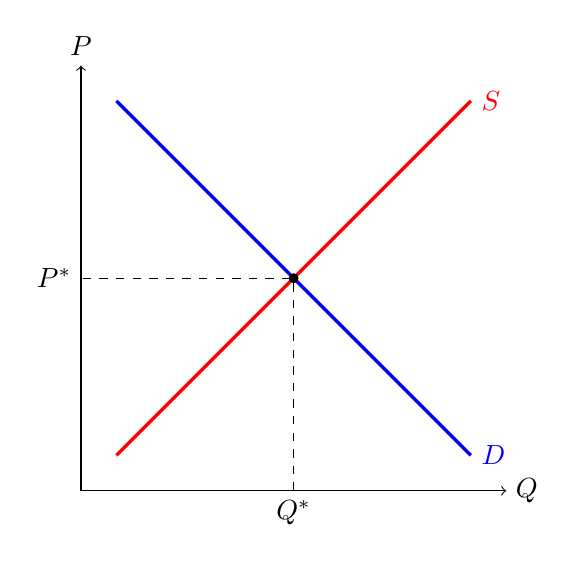
\begin{tikzpicture}[scale=0.9]
  \draw[->] (0,0) -- (6,0) node[right] {$Q$};
  \draw[->] (0,0) -- (0,6) node[above] {$P$};
  \draw[blue, very thick] (0.5,5.5) -- (5.5,0.5) node[right] {$D$};
  \draw[red,  very thick] (0.5,0.5) -- (5.5,5.5) node[right] {$S$};
  \fill (3,3) circle (2pt);
  \draw[dashed] (3,0) node[below]{$Q^*$} -- (3,3) -- (0,3) node[left]{$P^*$};
\end{tikzpicture}
\end{document}

  \end{center}
\end{frame}

% % main_lecture.tex（Beamer）
% \begin{frame}{経済成長と景気循環}
%   \begin{center}
%     % ============================================================
%  fig_business_cycle.tex
%  景気循環（Cycle）と経済成長（Trend）の概念図
%
%  【単体コンパイル】
%    uplatex  fig_business_cycle.tex
%    dvipdfmx fig_business_cycle.dvi
%
%  【Beamer への組み込み】
%    プリアンブルに \usepackage{standalone} を追加し
%    \input{fig_business_cycle} で呼び出す
%
%  パネル構成:
%    (a) 上段: 実際の GDP とトレンド（対数スケール）
%    (b) 下段: 循環成分のみ（トレンドからの乖離）
%
%  使用マクロ:
%    T(x)  = 0.55x + 1.5            （トレンド）
%    Y(x)  = T(x) + 0.7*sin(1.8x + 0.3)  （GDP）
%    C(x)  = 0.7*sin(1.8x + 0.3)         （循環成分）
%
%  主要座標（数値は解析的に計算）:
%    Peak  : x = 0.706, 4.197, 7.688
%    Trough: x = 2.451, 5.942, 9.433
% ============================================================
\documentclass[tikz, dvipdfmx]{standalone}
\usepackage{tikz}
\usepackage{pgfplots}
\pgfplotsset{compat=1.18}
\usepgfplotslibrary{groupplots, fillbetween}
\usetikzlibrary{arrows.meta}

% ── カラー定義 ──────────────────────────────────────────────
\definecolor{gdpblue}{RGB}{30, 90, 180}
\definecolor{trendred}{RGB}{190, 40, 40}
\definecolor{expgreen}{RGB}{200, 230, 200}
\definecolor{recred}{RGB}{240, 200, 200}

\begin{document}
\begin{tikzpicture}

\begin{groupplot}[
  group style={
    group size  = 1 by 2,
    vertical sep= 14mm,
  },
  width  = 12cm,
  xmin   = 0,   xmax = 10.5,
  xtick  = \empty,
  ytick  = \empty,
  axis lines      = left,
  axis line style = {thick},
  clip            = false,
  every axis plot/.append style = {smooth},
]

% ════════════════════════════════════════════════════════════
%  上段パネル: 実際の GDP とトレンド
% ════════════════════════════════════════════════════════════
\nextgroupplot[
  height = 6.5cm,
  ymin   = 0.5, ymax = 8.0,
  ylabel = {$\log Y_t$},
  ylabel style = {
    rotate  = -90,
    at      = {(axis description cs: -0.02, 1.0)},
    anchor  = south east,
    font    = \small,
  },
  title  = {\textbf{(a)}\; Actual GDP and Trend},
  title style = {
    at     = {(axis description cs: 0, 1)},
    anchor = south west,
    font   = \small\bfseries,
  },
]

  %% ── fill between 用の透明パス ────────────────────────────
  \addplot[draw=none, name path=gdp_path,
    domain=0:10, samples=300]
    { 0.55*x + 1.5 + 0.7*sin(deg(1.8*x + 0.3)) };

  \addplot[draw=none, name path=trend_path,
    domain=0:10, samples=2]
    { 0.55*x + 1.5 };

  %% ── 拡張局面（GDP > Trend）と後退局面（GDP < Trend）の塗りつぶし
  %%    x=0 で sin(0.3)>0 → GDP>Trend → segment 0 = even → green
  \addplot fill between[
    of = gdp_path and trend_path,
    every even segment/.style = {fill=expgreen},   % 拡張: 緑
    every odd  segment/.style = {fill=recred},     % 後退: 赤
  ];

  %% ── トレンド線（赤破線） ─────────────────────────────────
  \addplot[trendred, thick, dashed, domain=0:10, samples=2]
    { 0.55*x + 1.5 };
  %% トレンドのラベル
  \node[right, font=\footnotesize, trendred]
    at (axis cs: 10.05, 7.05) {Trend ($g$)};

  %% ── GDP 線（青） ────────────────────────────────────────
  \addplot[gdpblue, thick, domain=0:10, samples=300]
    { 0.55*x + 1.5 + 0.7*sin(deg(1.8*x + 0.3)) };
  %% GDP のラベル
  \node[right, font=\footnotesize, gdpblue]
    at (axis cs: 10.05, 7.85) {$Y_t$};

  %% ── Peak マーカー（●） ──────────────────────────────────
  %%    座標: (0.706, 2.588), (4.197, 4.508), (7.688, 6.428)
  \addplot[only marks, mark=*, mark size=2.5pt,
    mark options={fill=black, draw=black}]
    coordinates { (0.706, 2.588) (4.197, 4.508) (7.688, 6.428) };
  \node[above, font=\scriptsize] at (axis cs: 4.197, 4.508) {Peak};
  \node[above, font=\scriptsize] at (axis cs: 7.688, 6.428) {Peak};

  %% ── Trough マーカー（○） ─────────────────────────────────
  %%    座標: (2.451, 2.148), (5.942, 4.068)
  \addplot[only marks, mark=o, mark size=2.5pt,
    mark options={fill=white, draw=black, line width=1pt}]
    coordinates { (2.451, 2.148) (5.942, 4.068) };
  \node[below, font=\scriptsize] at (axis cs: 2.451, 2.148) {Trough};
  \node[below, font=\scriptsize] at (axis cs: 5.942, 4.068) {Trough};

  %% ── 循環成分の振れ幅を示す両矢印 ────────────────────────
  %%    x = 4.7 付近（Peak x=4.197 の右）に描画
  %%    trend(4.7)  = 0.55*4.7+1.5 = 4.085
  %%    GDP(4.7)    ≈ 4.085 + 0.7*sin(8.76) ≈ 4.085 + 0.629 = 4.714
  \draw[<->, thick, orange!80!black, >=Stealth]
    (axis cs: 4.75, 4.085) -- (axis cs: 4.75, 4.714);
  \node[right, font=\scriptsize, orange!80!black]
    at (axis cs: 4.80, 4.40) {Cycle};

  %% ── 成長率を示す矢印（トレンドに沿った傾き） ─────────────
  \draw[->, thick, trendred!60, >=Stealth]
    (axis cs: 6.5, 5.075) -- (axis cs: 8.0, 5.900);
  \node[below right, font=\scriptsize, trendred!80]
    at (axis cs: 7.0, 5.3) {slope $= g$};

  %% ── Expansion / Recession テキスト ───────────────────────
  \node[font=\scriptsize, gdpblue!80!black]
    at (axis cs: 3.3, 4.2) {\textit{Expansion}};
  \node[font=\scriptsize, trendred!80!black]
    at (axis cs: 1.6, 3.8) {\textit{Recession}};


% ════════════════════════════════════════════════════════════
%  下段パネル: 循環成分のみ
% ════════════════════════════════════════════════════════════
\nextgroupplot[
  height = 3.5cm,
  ymin   = -1.15, ymax = 1.5,
  ylabel = {Cyclical Component},
  ylabel style = {
    rotate  = -90,
    at      = {(axis description cs: -0.02, 1.0)},
    anchor  = south east,
    font    = \small,
  },
  xlabel = {Time $t$},
  xlabel style = {
    at     = {(axis description cs: 1.0, 0)},
    anchor = north east,
    font   = \small,
  },
  title  = {\textbf{(b)}\; Cyclical Component (Deviation from Trend)},
  title style = {
    at     = {(axis description cs: 0, 1)},
    anchor = south west,
    font   = \small\bfseries,
  },
]

  %% ── fill between 用の透明パス ────────────────────────────
  \addplot[draw=none, name path=cycle_path,
    domain=0:10, samples=300]
    { 0.7*sin(deg(1.8*x + 0.3)) };
  \addplot[draw=none, name path=zero_path,
    domain=0:10]
    { 0 };

  %% ── 拡張（正）/ 後退（負）の塗りつぶし ──────────────────
  \addplot fill between[
    of = cycle_path and zero_path,
    every even segment/.style = {fill=expgreen},
    every odd  segment/.style = {fill=recred},
  ];

  %% ── ゼロ基準線 ───────────────────────────────────────────
  \addplot[gray!60, thin, domain=0:10] { 0 }
    node[right, font=\scriptsize, gray] {Trend};

  %% ── 循環成分の線 ─────────────────────────────────────────
  \addplot[gdpblue, thick, domain=0:10, samples=300]
    { 0.7*sin(deg(1.8*x + 0.3)) };

  %% ── Peak マーカー ────────────────────────────────────────
  \addplot[only marks, mark=*, mark size=2pt,
    mark options={fill=black, draw=black}]
    coordinates { (0.706, 0.7) (4.197, 0.7) (7.688, 0.7) };

  %% ── Trough マーカー ─────────────────────────────────────
  \addplot[only marks, mark=o, mark size=2pt,
    mark options={fill=white, draw=black, line width=1pt}]
    coordinates { (2.451, -0.7) (5.942, -0.7) (9.433, -0.7) };

  %% ── Expansion / Recession ラベル ─────────────────────────
  \node[font=\scriptsize, gdpblue!80!black]
    at (axis cs: 0.353, 0.92) {\textit{Exp.}};
  \node[font=\scriptsize, trendred!80!black]
    at (axis cs: 2.45,  -0.95) {\textit{Rec.}};
  \node[font=\scriptsize, gdpblue!80!black]
    at (axis cs: 3.82,  0.92) {\textit{Exp.}};
  \node[font=\scriptsize, trendred!80!black]
    at (axis cs: 5.942, -0.95) {\textit{Rec.}};
  \node[font=\scriptsize, gdpblue!80!black]
    at (axis cs: 7.38,  0.92) {\textit{Exp.}};

\end{groupplot}

\end{tikzpicture}
\end{document}

%   \end{center}
% \end{frame}

% main_lecture.tex（Beamer）
% \begin{frame}{経済成長と景気循環}
%   \begin{center}
%     \input{tikz/Fig_bc_compact}
%   \end{center}
% \end{frame}

% 経済成長と景気循環の関係（TikZ）
\begin{frame}{経済成長と景気循環}
  \begin{center}
    % ============================================================
%  tikz_fig_bc_trend.tex  ── 上段パネルのみ（スライド1枚目用）
%  【使用例】
%    \begin{frame}{経済成長とトレンド}
%      \input{tikz/tikz_fig_bc_trend}
%    \end{frame}
% ============================================================
\documentclass[tikz, dvipdfmx]{standalone}
\usepackage{tikz}
\usepackage{pgfplots}
\pgfplotsset{compat=1.18}
\usepgfplotslibrary{fillbetween}
\usetikzlibrary{arrows.meta}
\definecolor{gdpblue} {RGB}{30,  90,  180}
\definecolor{trendred}{RGB}{190, 40,  40}
\definecolor{expgreen}{RGB}{200, 230, 200}
\definecolor{recred}  {RGB}{240, 200, 200}

\begin{document}
\begin{tikzpicture}
\begin{axis}[
  width  = \linewidth,
  height = 6.5cm,
  xmin = 0, xmax = 10.5,
  ymin = 0.5, ymax = 8.5,
  xtick = \empty, ytick = \empty,
  axis lines      = left,
  axis line style = {thick},
  clip            = false,
  every axis plot/.append style = {smooth},
  font = \small,
  ylabel = {$\log Y_t$},
  ylabel style = {
    rotate = -90,
    at     = {(axis description cs: -0.01, 1.0)},
    anchor = south east,
  },
  xlabel = {Time $t$},
  xlabel style = {
    at     = {(axis description cs: 1.0, 0)},
    anchor = north east,
  },
]
  % ── fill between 用透明パス ─────────────────────────────
  \addplot[draw=none, name path=gdp_path, domain=0:10, samples=300]
    { 0.55*x + 1.5 + 0.7*sin(deg(1.8*x + 0.3)) };
  \addplot[draw=none, name path=trend_path, domain=0:10, samples=2]
    { 0.55*x + 1.5 };

  % ── 拡張（緑）/ 後退（赤）シェーディング ────────────────
  \addplot fill between[
    of = gdp_path and trend_path,
    every even segment/.style = {fill=expgreen},
    every odd  segment/.style = {fill=recred},
  ];

  % ── トレンド線 ───────────────────────────────────────────
  \addplot[trendred, thick, dashed, domain=0:10, samples=2]
    { 0.55*x + 1.5 };
  \node[right, font=\small, trendred]
    at (axis cs: 10.05, 7.1) {Trend};
  % 成長率の傾き矢印
  \draw[->, thick, trendred!60, >=Stealth]
    (axis cs: 6.0, 4.8) -- (axis cs: 8.2, 6.0);
  \node[below right, font=\scriptsize, trendred!80]
    at (axis cs: 6.8, 5.1) {slope $= g$};

  % ── GDP 線 ──────────────────────────────────────────────
  \addplot[gdpblue, thick, domain=0:10, samples=300]
    { 0.55*x + 1.5 + 0.7*sin(deg(1.8*x + 0.3)) };
  \node[right, font=\small, gdpblue]
    at (axis cs: 10.05, 8.0) {$Y_t$};

  % ── Peak ● ──────────────────────────────────────────────
  \addplot[only marks, mark=*, mark size=2.5pt,
    mark options={fill=black}]
    coordinates { (0.706,2.588) (4.197,4.508) (7.688,6.428) };
  \node[above, font=\scriptsize] at (axis cs: 4.197, 4.508) {Peak};
  \node[above, font=\scriptsize] at (axis cs: 7.688, 6.428) {Peak};

  % ── Trough ○ ─────────────────────────────────────────────
  \addplot[only marks, mark=o, mark size=2.5pt,
    mark options={fill=white, draw=black, line width=1pt}]
    coordinates { (2.451,2.148) (5.942,4.068) };
  \node[below, font=\scriptsize] at (axis cs: 2.451, 2.148) {Trough};
  \node[below, font=\scriptsize] at (axis cs: 5.942, 4.068) {Trough};

  % ── 循環成分の振れ幅（両矢印） ──────────────────────────
  \draw[<->, thick, orange!80!black, >=Stealth]
    (axis cs: 4.75, 4.085) -- (axis cs: 4.75, 4.714);
  \node[right, font=\scriptsize, orange!80!black]
    at (axis cs: 4.80, 4.40) {Cycle};

  % ── Expansion / Recession ラベル ─────────────────────────
  \node[font=\small, gdpblue!80!black]
    at (axis cs: 3.3, 4.35) {\textit{Expansion}};
  \node[font=\small, trendred!80!black]
    at (axis cs: 1.6, 4.0) {\textit{Recession}};

\end{axis}
\end{tikzpicture}
\end{document}

  \end{center}
\end{frame}

% 景気循環のイメージ（TikZ）
\begin{frame}{景気循環}
  \begin{center}
    % ============================================================
%  tikz_fig_bc_cycle.tex  ── 下段パネルのみ（スライド2枚目用）
%  【使用例】
%    \begin{frame}{景気循環}
%      \input{tikz/tikz_fig_bc_cycle}
%    \end{frame}
% ============================================================
\documentclass[tikz, dvipdfmx]{standalone}
\usepackage{tikz}
\usepackage{pgfplots}
\pgfplotsset{compat=1.18}
\usepgfplotslibrary{fillbetween}
\usetikzlibrary{arrows.meta}
\definecolor{gdpblue} {RGB}{30,  90,  180}
\definecolor{trendred}{RGB}{190, 40,  40}
\definecolor{expgreen}{RGB}{200, 230, 200}
\definecolor{recred}  {RGB}{240, 200, 200}

\begin{document}
\begin{tikzpicture}
\begin{axis}[
  width  = \linewidth,
  height = 6.5cm,
  xmin = 0, xmax = 10.5,
  ymin = -1.4, ymax = 1.8,
  xtick = \empty, ytick = \empty,
  axis lines      = left,
  axis line style = {thick},
  clip            = false,
  every axis plot/.append style = {smooth},
  font = \small,
  %ylabel = {Cyclical component ($\log Y_t - \mathrm{Trend}_t$)},
  ylabel = {$\log Y_t - \mathrm{Trend}_t$},
  ylabel style = {
    rotate = -90,
    at     = {(axis description cs: -0.01, 1.0)},
    anchor = south east,
    xshift = 1.2cm,
  },
  xlabel = {Time $t$},
  xlabel style = {
    at     = {(axis description cs: 1.0, 0)},
    anchor = north east,
  },
]
  % ── fill between 用透明パス ─────────────────────────────
  \addplot[draw=none, name path=cycle_path, domain=0:10, samples=300]
    { 0.7*sin(deg(1.8*x + 0.3)) };
  \addplot[draw=none, name path=zero_path, domain=0:10] { 0 };

  % ── 拡張（緑）/ 後退（赤）シェーディング ────────────────
  \addplot fill between[
    of = cycle_path and zero_path,
    every even segment/.style = {fill=expgreen},
    every odd  segment/.style = {fill=recred},
  ];

  % ── ゼロ基準線 ──────────────────────────────────────────
  \addplot[gray!70, thin, domain=0:10] { 0 };
  \node[right, font=\scriptsize, gray!80]
    at (axis cs: 10.05, 0) {Trend};

  % ── 循環成分の線 ─────────────────────────────────────────
  \addplot[gdpblue, thick, domain=0:10, samples=300]
    { 0.7*sin(deg(1.8*x + 0.3)) };

  % ── 振れ幅の注釈 ─────────────────────────────────────────
  % Peak(x=4.197)での両矢印
  \draw[<->, thick, orange!80!black, >=Stealth]
    (axis cs: 4.6, 0) -- (axis cs: 4.6, 0.7);
  \node[right, font=\scriptsize, orange!80!black]
    at (axis cs: 4.65, 0.35) {Amplitude};

  % ── Peak ● ──────────────────────────────────────────────
  \addplot[only marks, mark=*, mark size=2.5pt,
    mark options={fill=black}]
    coordinates { (0.706,0.7) (4.197,0.7) (7.688,0.7) };
  \node[above, font=\scriptsize] at (axis cs: 0.706,  0.7) {Peak};
  \node[above, font=\scriptsize] at (axis cs: 4.197,  0.7) {Peak};
  \node[above, font=\scriptsize] at (axis cs: 7.688,  0.7) {Peak};

  % ── Trough ○ ─────────────────────────────────────────────
  \addplot[only marks, mark=o, mark size=2.5pt,
    mark options={fill=white, draw=black, line width=1pt}]
    coordinates { (2.451,-0.7) (5.942,-0.7) (9.433,-0.7) };
  \node[below, font=\scriptsize] at (axis cs: 2.451, -0.7) {Trough};
  \node[below, font=\scriptsize] at (axis cs: 5.942, -0.7) {Trough};

  % ── 周期を示す両矢印 ─────────────────────────────────────
  % Peak(0.706) → Peak(4.197) の間
  \draw[<->, semithick, black!60, >=Stealth]
    (axis cs: 0.706, -1.1) -- (axis cs: 4.197, -1.1);
  \node[below, font=\scriptsize, black!70]
    at (axis cs: 2.45, -1.1) {Period};

  % ── Expansion / Recession ラベル ─────────────────────────
  \node[font=\small, gdpblue!80!black]
    at (axis cs: 0.353,  1.1) {\textit{Expansion}};
  \node[font=\small, trendred!80!black]
    at (axis cs: 2.45,  -1.1) {};  % Periodラベルと重なるので省略
  \node[font=\small, gdpblue!80!black]
    at (axis cs: 3.82,   1.1) {\textit{Expansion}};
  \node[font=\small, trendred!80!black]
    at (axis cs: 5.942, -1.1) {};
  \node[font=\small, gdpblue!80!black]
    at (axis cs: 7.38,   1.1) {\textit{Expansion}};

  % Recession ラベル（Periodラベルと重ならない位置に）
  \node[font=\small, trendred!80!black]
    at (axis cs: 6.9, -1.05) {\textit{Recession}};

\end{axis}
\end{tikzpicture}
\end{document}

  \end{center}
\end{frame}

% 長期における総需要・総供給分析（TikZ）
\begin{frame}{総需要・総供給分析：長期均衡}
  \begin{center}
    \scalebox{0.8}{% ============================================================
%  tikz_fig_adas_lr.tex
%  長期の総需要・総供給（AD-AS）分析
%
%  【単体コンパイル】
%    uplatex  tikz_fig_adas_lr.tex && dvipdfmx tikz_fig_adas_lr.dvi
%
%  【Beamer への組み込み（my_preamble.tex に standalone 追加済みの場合）】
%    \input{tikz/tikz_fig_adas_lr}
%
%  曲線の仕様:
%    AD  : P = 10/Y + 1.5   （右下がり双曲線）
%    LRAS: Y = Y*  = 5.0    （垂直線・潜在 GDP）
%    均衡: (Y*, P*) = (5, 3.5)
%
%  コメントアウトで以下も用意:
%    SRAS : 短期総供給曲線（右上がり）
%    AD'  : 総需要曲線のシフト後（ADシフトの例）
% ============================================================
\documentclass[tikz, dvipdfmx]{standalone}
\usepackage{tikz}
\usetikzlibrary{arrows.meta}
\definecolor{gdpblue} {RGB}{30,  90,  180}
\definecolor{trendred}{RGB}{190, 40,  40}
\definecolor{srasgreen}{RGB}{30, 140, 60}

\begin{document}
\begin{tikzpicture}[
  >=Stealth,
  thick,
  % 1 unit = 1 cm; 図全体の描画域はおよそ 9.5 cm × 7.5 cm
]

% ── 軸 ──────────────────────────────────────────────────────
\draw[->] (0,0) -- (9.8,0)
  node[right, font=\small] {$Y$ (Output)};
\draw[->] (0,0) -- (0,7.8)
  node[above, font=\small] {$P$ (Price level)};

% ── 長期総供給曲線 LRAS（垂直線） ────────────────────────
%    Y = Y*（潜在 GDP）
\draw[trendred, very thick] (5,0) -- (5,7.2)
  node[above, font=\small, trendred] {LRAS};

% ── 総需要曲線 AD（右下がり） ─────────────────────────────
%    P = 10/Y + 1.5
%    Y*=5 のとき P* = 10/5 + 1.5 = 3.5
%    domain: P=7.4 → Y≈1.71,  P→1.5（漸近）→ Y→∞
\draw[gdpblue, very thick]
  plot[domain=1.72:9.3, samples=120, smooth] (\x, {10/\x + 1.5})
  node[right, font=\small, gdpblue] {AD};

% ── 均衡点 (Y*, P*) = (5, 3.5) ────────────────────────────
\fill[black] (5,3.5) circle[radius=2.5pt];

% ── P* への水平点線 ──────────────────────────────────────
\draw[dashed, gray!70, thin]
  (0,3.5) node[left, font=\small, black] {$P^*$} -- (5,3.5);

% ── Y* のラベル（横軸下）────────────────────────────────
\node[below, font=\small] at (5,0) {$Y^*$};


% ════════════════════════════════════════════════════════════
%  以下はコメントアウト:  必要に応じて有効化
% ════════════════════════════════════════════════════════════

%% ── (A) 短期総供給曲線 SRAS（右上がり）──────────────────
%%    短期均衡を示したい場合に有効化
%% \draw[srasgreen, very thick]
%%   plot[domain=0.3:9, samples=2, smooth] (\x, {0.7*\x + 0.0})
%%   node[right, font=\small, srasgreen] {SRAS};

%% ── (B) AD シフト（例: 拡張的財政・金融政策） ────────────
%%    AD が右上にシフト → 長期では P のみ上昇, Y は不変
%%
%%    AD' : P = 14/Y + 1.5   （AD を上方シフト）
%%    新均衡: (Y*, P**) = (5, 14/5+1.5) = (5, 4.3)
%%
%% % AD' 曲線
%% \draw[gdpblue!50, very thick, dashed]
%%   plot[domain=1.72:9.3, samples=120, smooth] (\x, {14/\x + 1.5})
%%   node[right, font=\small, gdpblue!70] {AD$'$};
%%
%% % 新均衡点
%% \fill[black] (5,4.3) circle[radius=2.5pt];
%%
%% % P** への水平点線
%% \draw[dashed, gray!70, thin]
%%   (0,4.3) node[left, font=\small, black] {$P^{**}$} -- (5,4.3);
%%
%% % AD から AD' へのシフト矢印
%% \draw[->, thick, gdpblue!60]
%%   (3.5, {10/3.5+1.5}+0.15) -- (3.5, {14/3.5+1.5}-0.15);

\end{tikzpicture}
\end{document}
}
  \end{center}
\end{frame}

% 総需要曲線のシフト（TikZ）
\begin{frame}{総需要・総供給分析：長期均衡}
  \begin{center}
    \scalebox{0.8}{% ============================================================
%  tikz_fig_adas_lr_shift.tex
%  長期 AD-AS：総需要シフトの効果
%
%  シナリオ: 拡張的財政・金融政策 → AD が右上にシフト
%  長期均衡: 実質 GDP は Y* に戻る（物価のみ P* → P** に上昇）
%  → 長期の「金融中立性」「古典派の二分法」の図解に使用
%
%  曲線の仕様:
%    AD  : P = 10/Y + 1.5  （シフト前）
%    AD' : P = 14/Y + 1.5  （シフト後）
%    LRAS: Y = Y* = 5.0
%    均衡1: (5, 3.5)  ←シフト前
%    均衡2: (5, 4.3)  ←シフト後
% ============================================================
\documentclass[tikz, dvipdfmx]{standalone}
\usepackage{tikz}
\usetikzlibrary{arrows.meta}
\definecolor{gdpblue} {RGB}{30,  90,  180}
\definecolor{trendred}{RGB}{190, 40,  40}

\begin{document}
\begin{tikzpicture}[
  >=Stealth,
  thick,
]

% ── 軸 ──────────────────────────────────────────────────────
\draw[->] (0,0) -- (9.8,0)
  node[right, font=\small] {$Y$ (Output)};
\draw[->] (0,0) -- (0,7.8)
  node[above, font=\small] {$P$ (Price level)};

% ── LRAS（垂直線） ────────────────────────────────────────
\draw[trendred, very thick] (5,0) -- (5,7.2)
  node[above, font=\small, trendred] {LRAS};

% ── AD（シフト前, 実線） ─────────────────────────────────
\draw[gdpblue, very thick]
  plot[domain=1.72:9.3, samples=120, smooth] (\x, {10/\x + 1.5})
  node[right, font=\small, gdpblue] {AD};

% ── AD'（シフト後, 破線） ────────────────────────────────
%    P = 14/Y + 1.5; 新均衡 (5, 4.3)
\draw[gdpblue, very thick, dashed]
  plot[domain=2.2:9.3, samples=120, smooth] (\x, {14/\x + 1.5})
  node[right, font=\small, gdpblue] {AD$'$};

% ── シフト矢印（ADからAD'へ） ────────────────────────────
%    曲線の中間あたりに矢印
\draw[->, thick, gdpblue!70]
  (3.3, {10/3.3 + 1.5 + 0.2}) -- (3.3, {14/3.3 + 1.5 - 0.2});

% ── 均衡点1（シフト前） ──────────────────────────────────
\fill[black]  (5, 3.5) circle[radius=2.5pt];
\node[left, font=\scriptsize, xshift=-2pt] at (5,3.5) {$E$};

% ── 均衡点2（シフト後） ──────────────────────────────────
\fill[black]  (5, 4.3) circle[radius=2.5pt];
\node[left, font=\scriptsize, xshift=-2pt] at (5,4.3) {$E'$};

% ── P* への水平点線（シフト前） ──────────────────────────
\draw[dashed, gray!70, thin]
  (0, 3.5) node[left, font=\small, black] {$P^*$} -- (5, 3.5);

% ── P** への水平点線（シフト後） ─────────────────────────
\draw[dashed, gray!70, thin]
  (0, 4.3) node[left, font=\small, black] {$P^{**}$} -- (5, 4.3);

% ── 物価上昇の縦矢印 ─────────────────────────────────────
\draw[<->, semithick, black!60]
  (0.6, 3.5) -- (0.6, 4.3);

% ── Y* ───────────────────────────────────────────────────
\node[below, font=\small] at (5,0) {$Y^*$};

% ── 「実質 GDP は不変」の注釈 ────────────────────────────
\node[
  align  = center,
  font   = \scriptsize,
  black!70,
] at (7.5, 1.5) {$\Delta Y = 0$ in LR\\(only $P$ rises)};

\end{tikzpicture}
\end{document}
}
  \end{center}
\end{frame}

% 短期における総需要・総供給分析（TikZ）
\begin{frame}{総需要・総供給分析：短期均衡}
  \begin{center}
    \scalebox{0.8}{% ============================================================
%  tikz_fig_adas_sr.tex
%  短期の総需要・総供給（Short-Run AD-AS）分析
%
%  【単体コンパイル】
%    uplatex  tikz_fig_adas_sr.tex && dvipdfmx tikz_fig_adas_sr.dvi
%
%  【Beamer への組み込み】
%    my_preamble.tex に以下を追加してから \input{tikz/tikz_fig_adas_sr}
%      \definecolor{srasgreen}{RGB}{30, 140, 60}
%
%  曲線の仕様:
%    AD  : P = 10/Y + 1.5   （右下がり双曲線）
%    SRAS: P = 0.5Y + 1     （右上がり直線; 価格粘着性）
%    均衡: (Y₀, P₀) = (5, 3.5)
%
%  ※ 長期版（tikz_fig_adas_lr.tex）と座標系・スタイルを統一済み
%    → 同じスライドセットに並べて使用可能
%
%  コメントアウトで以下も用意:
%    (A) AD シフト（拡張的需要政策 → P↑, Y↑）
%    (B) SRAS 上方シフト（負のサプライショック → スタグフレーション）
%    (C) SRAS 下方シフト（正のサプライショック → P↓, Y↑）
% ============================================================
\documentclass[tikz, dvipdfmx]{standalone}
\usepackage{tikz}
\usetikzlibrary{arrows.meta}
\definecolor{gdpblue}  {RGB}{30,  90,  180}
\definecolor{srasgreen}{RGB}{30, 140,  60}

\begin{document}
\begin{tikzpicture}[
  >=Stealth,
  thick,
]

% ── 軸 ──────────────────────────────────────────────────────
\draw[->] (0,0) -- (9.8,0)
  node[right, font=\small] {$Y$ (Output)};
\draw[->] (0,0) -- (0,7.8)
  node[above, font=\small] {$P$ (Price level)};

% ── 短期総供給曲線 SRAS（右上がり） ──────────────────────
%    P = 0.5Y + 1
%    右上がりの根拠: 価格・賃金の粘着性（短期では名目賃金固定）
%    Y=0.2→P=1.1,  Y=5→P=3.5,  Y=8.5→P=5.25
\draw[srasgreen, very thick]
  plot[domain=0.2:8.5, samples=2] (\x, {0.5*\x + 1})
  node[right, font=\small, srasgreen] {SRAS};

% ── 総需要曲線 AD（右下がり） ─────────────────────────────
%    P = 10/Y + 1.5
%    右下がりの根拠: 富の効果, 利子率効果, 為替レート効果
%    Y≈1.72→P≈7.3,  Y=5→P=3.5,  Y=9.3→P≈2.6
\draw[gdpblue, very thick]
  plot[domain=1.72:9.3, samples=120, smooth] (\x, {10/\x + 1.5})
  node[right, font=\small, gdpblue] {AD};

% ── 短期均衡点 (Y₀, P₀) = (5, 3.5) ────────────────────────
%    AD ∩ SRAS:  10/Y + 1.5 = 0.5Y + 1
%                → Y² - Y - 20 = 0 → Y = 5 ✓
\fill[black] (5, 3.5) circle[radius=2.5pt];

% ── 均衡値への点線 ───────────────────────────────────────
\draw[dashed, gray!70, thin]
  (0, 3.5) node[left, font=\small, black] {$P_0$} -- (5, 3.5);
\draw[dashed, gray!70, thin]
  (5, 0)   node[below, font=\small, black] {$Y_0$} -- (5, 3.5);


% ════════════════════════════════════════════════════════════
%  以下はコメントアウト: 必要に応じて有効化
% ════════════════════════════════════════════════════════════

%% ── (A) AD 右シフト（拡張的財政・金融政策） ─────────────
%%    AD' : P = 14/Y + 1.5
%%    新均衡: Y₁ ≈ 6.52, P₁ ≈ 4.26  ← 短期では Y も上昇（長期と違う!）
%%
%% \draw[gdpblue!60, very thick, dashed]
%%   plot[domain=2.2:9.3, samples=120, smooth] (\x, {14/\x + 1.5})
%%   node[right, font=\small, gdpblue!70] {AD$'$};
%% % 新均衡点
%% \fill[black] (6.52, 4.26) circle[radius=2pt];
%% \draw[dashed, gray!50, thin] (0, 4.26) -- (6.52, 4.26)
%%   node[above left, font=\scriptsize] {};
%% \draw[dashed, gray!50, thin] (6.52, 0) node[below, font=\scriptsize] {$Y_1$}
%%   -- (6.52, 4.26);
%% \node[left, font=\scriptsize] at (0, 4.26) {$P_1$};
%% % シフト矢印
%% \draw[->, thick, gdpblue!60]
%%   (3.0, {10/3.0+1.5+0.2}) -- (3.0, {14/3.0+1.5-0.2});

%% ── (B) SRAS 上方シフト（負のサプライショック: 原油高など）
%%    スタグフレーション: P↑ かつ Y↓
%%    SRAS': P = 0.5Y + 2.5
%%    新均衡: Y₁ ≈ 3.58, P₁ ≈ 4.29
%%
%% \draw[srasgreen!60, very thick, dashed]
%%   plot[domain=0.2:8.5, samples=2] (\x, {0.5*\x + 2.5})
%%   node[right, font=\small, srasgreen!70] {SRAS$'$};
%% \fill[black] (3.58, 4.29) circle[radius=2pt];
%% \draw[dashed, gray!50, thin] (0, 4.29) node[left, font=\scriptsize] {$P_1$}
%%   -- (3.58, 4.29);
%% \draw[dashed, gray!50, thin] (3.58, 0) node[below, font=\scriptsize] {$Y_1$}
%%   -- (3.58, 4.29);
%% % シフト矢印
%% \draw[->, thick, srasgreen!60]
%%   (6.5, {0.5*6.5+1+0.15}) -- (6.5, {0.5*6.5+2.5-0.15});

%% ── (C) SRAS 下方シフト（正のサプライショック: 技術進歩など）
%%    P↓ かつ Y↑
%%    SRAS'': P = 0.5Y - 0.5
%%    新均衡: Y₁ ≈ 6.90, P₁ ≈ 2.95
%%
%% \draw[srasgreen!60, very thick, dashed]
%%   plot[domain=1.0:9.0, samples=2] (\x, {0.5*\x - 0.5})
%%   node[right, font=\small, srasgreen!70] {SRAS$''$};
%% \fill[black] (6.90, 2.95) circle[radius=2pt];
%% \draw[dashed, gray!50, thin] (0, 2.95) node[left, font=\scriptsize] {$P_1$}
%%   -- (6.90, 2.95);
%% \draw[dashed, gray!50, thin] (6.90, 0) node[below, font=\scriptsize] {$Y_1$}
%%   -- (6.90, 2.95);

\end{tikzpicture}
\end{document}
}
  \end{center}
\end{frame}

% 因果推論（TikZ）
\begin{frame}{政策評価がなぜ難しいのか？：因果推論の根本問題}
  \begin{center}
    \scalebox{0.8}{% ============================================================
%  tikz_fig_causal_simple.tex
%  因果推論の根本問題（シンプル版）
%  「政策あり」か「なし」のどちらか一方しか観測できない
% ============================================================
\documentclass[tikz, dvipdfmx]{standalone}
\usepackage{tikz}
\usetikzlibrary{arrows.meta}
\definecolor{gdpblue}{RGB}{30,  90, 180}
\definecolor{obscol} {RGB}{210, 228, 255}   % 観測可能（薄青）
\definecolor{cfcol}  {RGB}{232, 232, 232}   % 観測不可（薄灰）

\begin{document}
\begin{tikzpicture}[>=Stealth, thick, every node/.style={font=\small}]

% ── 中心ノード（個人 or 地域） ───────────────────────────────
\node[
  draw=black!50, fill=black!6, rounded corners=5pt,
  minimum width=2.6cm, minimum height=0.9cm,
  align=center,
] (unit) at (0,0) {Individual $i$\\(or region $i$)};

% ── 上: 政策あり → 観測可能 ──────────────────────────────────
\draw[->, very thick, gdpblue]
  (unit.east) .. controls +(1.2,0) and +(-1.2,0) .. (4.5, 1.8)
  node[
    draw=gdpblue!60, fill=obscol,
    rounded corners=4pt,
    minimum width=5.0cm, minimum height=1.0cm,
    align=center, anchor=west,
  ] (obs) {$Y_i(1)$ \quad \textbf{Observable}\\
           {\scriptsize (outcome under policy)}};

% 矢印ラベル
\node[font=\scriptsize, gdpblue!80, above] at (2.2, 1.2)
  {With policy ($D_i = 1$)};

% ── 下: 政策なし → 観測不可能 ────────────────────────────────
\draw[->, very thick, dashed, black!35]
  (unit.east) .. controls +(1.2,0) and +(-1.2,0) .. (4.5,-1.8)
  node[
    draw=black!30, fill=cfcol,
    dashed, rounded corners=4pt,
    minimum width=5.0cm, minimum height=1.0cm,
    align=center, anchor=west,
  ] (cf) {$Y_i(0)$ \quad \textbf{Unobservable}\\
          {\scriptsize (counterfactual)}};

% 矢印ラベル
\node[font=\scriptsize, black!50, below] at (2.2,-1.2)
  {Without policy ($D_i = 0$)};

% ── 処置効果の注釈 ───────────────────────────────────────────
\node[
  draw=black!30, fill=black!4, rounded corners=4pt,
  font=\small, align=center,
] at (7.3, 0)
  {Causal effect:\\[4pt]
   $\tau_i = Y_i(1) - Y_i(0)$\\[4pt]
   {\small$= \;?\;$ (never observed)}};

% ── 「どちらか一方しか見えない」矢印 ─────────────────────────
\draw[<->, semithick, black!40]
  (obs.east) -- (7.3, 1.8);
\draw[<->, semithick, black!40]
  (cf.east)  -- (7.3,-1.8);

% ── 下部メッセージ ────────────────────────────────────────────
\node[font=\small, black!60, align=center] at (4.5, -3.2)
  {\textbf{Only one state is ever observed.}\\
   This is the \emph{Fundamental Problem of Causal Inference}.};

\end{tikzpicture}
\end{document}
}
  \end{center}
\end{frame}

% 景気対策の評価（TikZ）
\begin{frame}{政策評価がなぜ難しいのか？：景気対策の評価}
  \begin{center}
    \scalebox{0.8}{% ============================================================
%  Fig_counterfactual_cycle.tex
%  因果推論：反実仮想によるビジネスサイクルと政策効果
%  「政策なしなら、もっと悪化していた」を示すtime-series図
%  upLaTeX + dvipdfmx / standalone
% ============================================================
\documentclass[tikz, dvipdfmx]{standalone}
\usepackage{tikz}
\usetikzlibrary{arrows.meta, decorations.pathreplacing, calligraphy}

% ── 色定義（Fig_causal_simple.tex と統一） ──────────────────
\definecolor{gdpblue}{RGB}{30,  90, 180}   % 観測軌跡
\definecolor{obscol} {RGB}{210, 228, 255}  % 観測可能（薄青）
\definecolor{cfcol}  {RGB}{232, 232, 232}  % 観測不可（薄灰）
\definecolor{fillcol}{RGB}{180, 215, 255}  % 政策効果の差分領域

\begin{document}
\begin{tikzpicture}[
  >=Stealth,
  thick,
  every node/.style={font=\small},
  % 単位: 1 = 1cm
]

% ============================================================
%  0.  差分領域（一番先に描いてから線を上書き）
% ============================================================
\fill[fillcol, opacity=0.45]
  % 観測軌跡（政策あり）：前進方向
  plot[smooth, tension=0.5] coordinates {
    (4.0, 3.80)
    (4.8, 3.45)
    (5.5, 3.15)
    (6.0, 3.00)
    (6.8, 3.05)
    (7.5, 3.35)
    (8.3, 3.75)
    (9.0, 4.05)
    (9.8, 4.20)
  }
  % 反実仮想（政策なし）：逆順でパスを閉じる
  -- plot[smooth, tension=0.5] coordinates {
    (9.8, 2.20)
    (9.0, 2.00)
    (8.3, 1.75)
    (7.5, 1.45)
    (6.8, 1.40)
    (6.0, 1.65)
    (5.5, 2.10)
    (4.8, 3.10)
    (4.0, 3.80)
  } -- cycle;

% ============================================================
%  1.  座標軸
% ============================================================
% 横軸
\draw[->, thick, black!70]
  (-0.2, 0) -- (10.8, 0)
  node[right, font=\small] {Time};

% 縦軸
\draw[->, thick, black!70]
  (0, -0.3) -- (0, 5.2)
  node[above, font=\small, align=center] {Economic\\Activity};

% 縦軸の High / Low ラベル
\node[font=\scriptsize, black!50, left] at (0, 4.8) {High};
\node[font=\scriptsize, black!50, left] at (0, 0.5) {Low};

% ============================================================
%  2.  政策前の共通軌跡（t = 0 → 4）
%      緩やかな成長からピーク、危機の予兆へ
% ============================================================
\draw[black!60, very thick, line cap=round]
  plot[smooth, tension=0.5] coordinates {
    (0.0, 2.50)
    (0.7, 2.75)
    (1.3, 3.05)
    (2.0, 3.35)
    (2.8, 3.65)
    (3.4, 3.85)
    (3.8, 3.90)
    (4.0, 3.80)
  };

% ============================================================
%  3.  政策介入点（t = 4）の縦線
% ============================================================
\draw[dashed, black!40, thin]
  (4.0, -0.15) -- (4.0, 4.80);

\node[font=\scriptsize, black!60, align=center, below]
  at (4.0, -0.15)
  {Policy\\Intervention};

% ============================================================
%  4.  観測軌跡（政策あり、t = 4 → 9.8）  実線・青
% ============================================================
\draw[gdpblue, very thick, line cap=round]
  plot[smooth, tension=0.5] coordinates {
    (4.0, 3.80)
    (4.8, 3.45)
    (5.5, 3.15)
    (6.0, 3.00)
    (6.8, 3.05)
    (7.5, 3.35)
    (8.3, 3.75)
    (9.0, 4.05)
    (9.8, 4.20)
  };

% 観測軌跡ラベルボックス
\node[
  draw=gdpblue!70, fill=obscol,
  rounded corners=4pt,
  minimum width=4.0cm, minimum height=0.9cm,
  align=center, anchor=west, font=\small,
] (obs_box) at (10.0, 4.20)
  {$Y(1)$ \quad \textbf{Observable}\\
   {\scriptsize (with policy)}};

% ============================================================
%  5.  反実仮想（政策なし、t = 4 → 9.8）  破線・グレー
% ============================================================
\draw[black!40, very thick, dashed, line cap=round]
  plot[smooth, tension=0.5] coordinates {
    (4.0, 3.80)
    (4.8, 3.10)
    (5.5, 2.10)
    (6.0, 1.65)
    (6.8, 1.40)
    (7.5, 1.45)
    (8.3, 1.75)
    (9.0, 2.00)
    (9.8, 2.20)
  };

% 反実仮想ラベルボックス
\node[
  draw=black!35, fill=cfcol,
  dashed, rounded corners=4pt,
  minimum width=4.0cm, minimum height=0.9cm,
  align=center, anchor=west, font=\small,
] (cf_box) at (10.0, 2.20)
  {$Y(0)$ \quad \textbf{Unobservable}\\
   {\scriptsize (without policy)}};

% ============================================================
%  6.  "Today" マーカー（t = 9）
% ============================================================
\draw[dashed, black!35, thin]
  (9.0, -0.15) -- (9.0, 4.40);

\node[font=\scriptsize, black!55, below]
  at (9.0, -0.15) {Today};

% 観測点（Today）のドット
\filldraw[gdpblue] (9.0, 4.05) circle (3pt);

% ============================================================
%  7.  Policy Effect の双方向矢印（t ≈ 7.5）
% ============================================================
% 矢印
\draw[<->, very thick, gdpblue!80]
  (7.5, 1.45) -- (7.5, 3.35);

% ラベル
\node[
  fill=white, draw=gdpblue!40,
  rounded corners=3pt,
  font=\scriptsize, gdpblue!90,
  align=center, anchor=west,
] at (7.65, 2.40)
  {\textbf{Policy}\\[1pt]\textbf{Effect}};

% 上端・下端の水平ティック
\draw[gdpblue!60, thin] (7.3, 3.35) -- (7.7, 3.35);
\draw[gdpblue!60, thin] (7.3, 1.45) -- (7.7, 1.45);

% ============================================================
%  8.  「現在の観測値」水平参照線（薄い）
% ============================================================
\draw[gdpblue!30, thin, dashed]
  (0.0, 4.05) -- (9.0, 4.05);
\node[font=\tiny, gdpblue!60, left] at (0.0, 4.05)
  {Observed level today};

\draw[black!20, thin, dashed]
  (0.0, 2.00) -- (9.0, 2.00);
\node[font=\tiny, black!45, left] at (0.0, 2.00)
  {Counterfactual level};

% ============================================================
%  9.  下部メッセージボックス
% ============================================================
\node[
  draw=black!30, fill=black!4,
  rounded corners=5pt,
  font=\small, align=center,
  minimum width=9.5cm,
] at (5.5, -1.1)
  {\textbf{The economy looks ``not so bad'' only because the policy worked.}\\[3pt]
   {\small Without intervention, the downturn would have been far deeper.}\\[2pt]
   {\scriptsize This gap — $Y(1) - Y(0)$ — is the \emph{causal effect}, but $Y(0)$ is never observed.}};

\end{tikzpicture}
\end{document}
}
  \end{center}
\end{frame}

% DiD（TikZ）
\begin{frame}{Difference-in-Differences 分析のイメージ}
  \begin{center}
    \scalebox{0.8}{% ============================================================
%  tikz_fig_did.tex
%  Difference-in-Differences（DiD）の概念図
%
%  【単体コンパイル】
%    uplatex  tikz_fig_did.tex && dvipdfmx tikz_fig_did.dvi
%
%  【Beamer への組み込み】
%    \input{tikz/tikz_fig_did}
%
%  設定値:
%    Y_{C,0}   = 2.0  （対照群・処置前）
%    Y_{T,0}   = 4.5  （処置群・処置前）
%    Y_{C,1}   = 3.5  （対照群・処置後）
%    Y_{T,1}   = 7.5  （処置群・処置後・実績）
%    Y_{CF,1}  = 6.0  （処置群・処置後・反事実）
%                     = Y_{T,0} + (Y_{C,1} - Y_{C,0}) = 4.5 + 1.5
%
%    DiD = (Y_{T,1} - Y_{T,0}) - (Y_{C,1} - Y_{C,0})
%        = (7.5 - 4.5)         - (3.5 - 2.0)
%        = 3.0                 - 1.5          = 1.5
%
%  コメントアウトで以下も用意:
%    (A) 変化分解の縦矢印（ΔY_T, ΔY_C を右端に並置）
%    (B) DiD 公式テキスト
% ============================================================
\documentclass[tikz, dvipdfmx]{standalone}
\usepackage{tikz}
\usetikzlibrary{arrows.meta, decorations.pathreplacing}
\definecolor{gdpblue} {RGB}{30,  90,  180}
\definecolor{trendred}{RGB}{190, 40,  40}
\definecolor{cfgray}  {RGB}{100, 140, 200}   % 反事実（薄い青）

\begin{document}
\begin{tikzpicture}[
  >=Stealth,
  thick,
]

%% ─── 座標系 ────────────────────────────────────────────────
%%  横軸: x ∈ [0, 12]
%%  Pre 点  x = 2,  Post 点 x = 8,  Policy 縦線 x = 5
%%  縦軸: y ∈ [0, 9]

% ── 軸 ──────────────────────────────────────────────────────
\draw[->] (0,0) -- (12.2,0)
  node[right, font=\small] {Time};
\draw[->] (0,0) -- (0,9.5)
  node[above, font=\small] {$Y$ (Outcome)};

% ── Pre / Post ラベル ────────────────────────────────────────
\node[below=4pt, font=\small] at (2,0) {$t=0$};
\node[below=14pt, font=\scriptsize, gray] at (2,0) {(Pre-treatment)};
\node[below=4pt, font=\small] at (8,0) {$t=1$};
\node[below=14pt, font=\scriptsize, gray] at (8,0) {(Post-treatment)};

% ── Policy Implementation 縦破線 ────────────────────────────
\draw[gray!50, thin, dashed] (5,0) -- (5,9.2);
\node[above, font=\scriptsize, gray!80, align=center] at (5,9.2)
  {Policy\\Implemented};

% ── 縦軸の参照点（水平点線 + ラベル） ───────────────────────
% Y_{C,0} = 2.0
\draw[gray!35, thin, dashed] (0,2.0) -- (8.05,2.0);
\node[left, font=\scriptsize] at (-0.05,2.0) {$Y_{C,0}$};

% Y_{C,1} = 3.5
\draw[gray!35, thin, dashed] (0,3.5) -- (8.05,3.5);
\node[left, font=\scriptsize] at (-0.05,3.5) {$Y_{C,1}$};

% Y_{T,0} = 4.5
\draw[gray!35, thin, dashed] (0,4.5) -- (8.05,4.5);
\node[left, font=\scriptsize] at (-0.05,4.5) {$Y_{T,0}$};

% Y_{CF,1} = 6.0
\draw[gray!35, thin, dashed] (0,6.0) -- (8.05,6.0);
\node[left, font=\scriptsize] at (-0.05,6.0) {$Y_{CF,1}$};

% Y_{T,1} = 7.5
\draw[gray!35, thin, dashed] (0,7.5) -- (8.05,7.5);
\node[left, font=\scriptsize] at (-0.05,7.5) {$Y_{T,1}$};


% ════════════════════════════════════════════════════════════
%  主要曲線
% ════════════════════════════════════════════════════════════

% ── 対照群 Control（赤実線） ─────────────────────────────────
\draw[trendred, very thick] (2,2.0) -- (8,3.5);
\fill[trendred] (2,2.0) circle[radius=2.5pt];
\fill[trendred] (8,3.5) circle[radius=2.5pt];
\node[right, font=\small, trendred] at (8.15,3.5)
  {Control};

% ── 処置群 実績 Treatment actual（青実線） ───────────────────
\draw[gdpblue, very thick] (2,4.5) -- (8,7.5);
\fill[gdpblue] (2,4.5) circle[radius=2.5pt];
\fill[gdpblue] (8,7.5) circle[radius=2.5pt];
\node[right, font=\small, gdpblue] at (8.15,7.5)
  {Treatment (actual)};

% ── 反事実 Counterfactual（青系の破線）──────────────────────
%    傾き = 対照群と同じ = (3.5-2.0)/(8-2) = 0.25/unit
%    Y_{CF}(x) = 4.5 + 0.25*(x-2)
%    x=8 → Y_{CF,1} = 4.5 + 1.5 = 6.0 ✓
\draw[cfgray, very thick, dashed] (2,4.5) -- (8,6.0);
\fill[cfgray] (8,6.0) circle[radius=2.5pt];
\node[right, font=\small, cfgray] at (8.15,6.0)
  {Treatment (counterfactual)};


% ════════════════════════════════════════════════════════════
%  DiD 推定量のアノテーション
% ════════════════════════════════════════════════════════════

% ── DiD 縦の両矢印（Y_{CF,1} ↔ Y_{T,1}） ────────────────────
\draw[<->, very thick, orange!85!black]
  (9.3, 6.0) -- (9.3, 7.5);
\node[right, font=\small, orange!85!black, align=left]
  at (9.45, 6.75)
  {$\hat{\delta}^{\,\mathrm{DiD}} = 1.5$};

% ── 波括弧で DiD の範囲を強調 ─────────────────────────────
\draw[decorate,
  decoration={brace, amplitude=5pt, mirror},
  orange!85!black, semithick]
  (8.9, 6.0) -- (8.9, 7.5);

% ── Parallel Trends 注釈 ────────────────────────────────────
%    対照群と反事実の傾きが等しいことを示す
%    傾き = arctan(0.25) ≈ 14°
\node[font=\scriptsize, gray!80, rotate=14, align=center]
  at (5.5, 5.3)
  {Parallel Trends\\Assumption};


% ════════════════════════════════════════════════════════════
%  コメントアウト: 変化分解の縦矢印（右端に並置）
% ════════════════════════════════════════════════════════════

%% ── (A) ΔY_T（処置群の変化）: x=10.8 ──────────────────────
%% \draw[<->, semithick, gdpblue!80]
%%   (10.8, 4.5) -- (10.8, 7.5);
%% \draw[dashed, gray!30, thin] (0,4.5) -- (10.8,4.5);
%% \draw[dashed, gray!30, thin] (0,7.5) -- (10.8,7.5);
%% \node[right, font=\scriptsize, gdpblue!80] at (10.9, 6.0)
%%   {$\Delta Y_T = 3.0$};
%%
%% ── (B) ΔY_C（対照群の変化）: x=11.5 ──────────────────────
%% \draw[<->, semithick, trendred!80]
%%   (11.5, 2.0) -- (11.5, 3.5);
%% \node[right, font=\scriptsize, trendred!80] at (11.6, 2.75)
%%   {$\Delta Y_C = 1.5$};
%%
%% ── (C) DiD 公式テキスト ─────────────────────────────────
%% \node[align=left, font=\scriptsize, gray!80] at (9.5, 1.2) {%
%%   $\hat{\delta}^{\,\mathrm{DiD}}$
%%   $= \underbrace{(Y_{T,1}-Y_{T,0})}_{3.0}
%%      - \underbrace{(Y_{C,1}-Y_{C,0})}_{1.5} = 1.5$};

\end{tikzpicture}
\end{document}
}
  \end{center}
\end{frame}

% ストックとフローの関係（TikZ）
\begin{frame}{ストックとフローの関係}
  \begin{center}
    \scalebox{0.6}{% ============================================================
%  tikz_fig_flow_stock.tex
%  フロー（Flow）とストック（Stock）の概念図
%  バスタブ（bathtub）モデルで直感的に説明
%
%  ストック: ある時点での「残高・量」（水位）
%  フロー  : 単位時間あたりの「変化・移動」（流入・流出）
% ============================================================
\documentclass[tikz, dvipdfmx]{standalone}
\usepackage{tikz}
\usepackage{amsmath}
\usetikzlibrary{arrows.meta, decorations.pathreplacing}
\definecolor{gdpblue} {RGB}{30,  90, 180}
\definecolor{trendred}{RGB}{190,  40,  40}
\definecolor{watercol}{RGB}{175, 210, 240}

\begin{document}
\begin{tikzpicture}[
  >=Stealth, thick,
  every node/.style={font=\small},
]

% ============================================================
%  流入管（上部）
% ============================================================
\filldraw[fill=gdpblue!20, draw=gdpblue!50]
  (1.4, 4.0) rectangle (2.6, 5.8);

% 管の内側の矢印（水が流れるイメージ）
\draw[->, very thick, gdpblue!70]
  (2.0, 5.6) -- (2.0, 4.05);

% 流入ラベル（管の右側）
\node[right=4pt, gdpblue!80, font=\small\bfseries] at (2.7, 5.3)
  {Flow in};
\node[right=4pt, font=\scriptsize, gdpblue!60] at (2.7, 4.9)
  {(Investment $I_t$)};
\node[right=4pt, font=\scriptsize, black!40] at (2.7, 4.55)
  {\textit{measured per unit time}};

% ============================================================
%  バスタブ本体
% ============================================================

% 水（fill）
\fill[watercol!70] (0.0, 0.0) rectangle (4.0, 2.4);

% 水面
\draw[gdpblue!60, semithick] (0.0, 2.4) -- (4.0, 2.4);

% バスタブ外形（U字: 左・底・右の3辺）
\draw[black!65, very thick]
  (0.0, 4.2) -- (0.0, 0.0) -- (4.0, 0.0) -- (4.0, 4.2);

% ── ストックのラベル（タンク内）──────────────────────────────
\node[font=\large\bfseries, gdpblue] at (2.0, 1.5)
  {Stock};
\node[font=\small, gdpblue!70] at (2.0, 0.85)
  {Capital $K_t$};

% ── 空き領域のラベル ──────────────────────────────────────────
\node[font=\scriptsize, black!30] at (2.0, 3.3)
  {(unused capacity)};

% ── 水面の高さを示す波括弧（右側） ──────────────────────────
\draw[decorate,
  decoration={brace, amplitude=5pt},
  semithick, black!40]
  (4.2, 0.0) -- (4.2, 2.4);
\node[right=6pt, font=\small, black!60, align=left] at (4.2, 1.2)
  {$K_t$\\{\scriptsize (measured at}\\{\scriptsize a point in time)}};

% ============================================================
%  流出管（下部）
% ============================================================
\filldraw[fill=trendred!15, draw=trendred!45]
  (1.4, -1.8) rectangle (2.6, 0.0);

% 管の内側の矢印
\draw[->, very thick, trendred!65]
  (2.0, -0.05) -- (2.0, -1.65);

% 流出ラベル（管の右側）
\node[right=4pt, trendred!80, font=\small\bfseries] at (2.7, -0.8)
  {Flow out};
\node[right=4pt, font=\scriptsize, trendred!60] at (2.7, -1.2)
  {(Depreciation $\delta K_t$)};
\node[right=4pt, font=\scriptsize, black!40] at (2.7, -1.55)
  {\textit{measured per unit time}};

% ============================================================
%  恒等式ボックス（下部）
% ============================================================
\node[
  draw=black!25, fill=black!4, rounded corners=5pt,
  inner sep=8pt, align=center,
] at (2.0, -3.3) {%
  $\underbrace{K_{t+1}}_{\text{Stock (next period)}}$
  $\;=\;$
  $\underbrace{K_t}_{\text{Stock}}$
  $\;+\;$
  $\underbrace{I_t}_{\text{Flow in}}$
  $\;-\;$
  $\underbrace{\delta K_t}_{\text{Flow out}}$%
};

% ============================================================
%  右側: 経済学における例
% ============================================================
\node[font=\small\bfseries, black!70] at (10.0, 4.5)
  {Examples in Economics};
\draw[black!25, thin] (7.0, 4.2) -- (13.5, 4.2);

% ヘッダー行
\node[font=\small\bfseries, gdpblue]   at ( 8.8, 3.7) {Stock};
\node[font=\small\bfseries, black!50]  at (10.5, 3.7) {};
\node[font=\small\bfseries, trendred]  at (12.2, 3.7) {Flow};

\draw[black!20, thin] (7.0, 3.4) -- (13.5, 3.4);

% 各行
\foreach \i/\stk/\flw in {
  1/{Capital $K$}/{Investment $I$, Depreciation $\delta K$},
  2/{Population $N$}/{Births, Deaths},
  3/{Wealth $W$}/{Saving, Consumption},
  4/{Government debt}/{Budget deficit / surplus},
  5/{Water reservoir}/{Rainfall, Outflow}
} {
  \pgfmathsetmacro\ypos{3.0 - (\i-1)*0.75}
  \node[font=\small, align=left,  anchor=west] at (7.1, \ypos) {\stk};
  \node[font=\small, align=left,  anchor=west] at (10.3, \ypos) {\flw};
}

% 縦区切り線
\draw[black!20, thin] (10.1, 4.2) -- (10.1, -0.3);
\draw[black!20, thin] (7.0,  4.2) -- (7.0,  -0.3);
\draw[black!20, thin] (13.5, 4.2) -- (13.5, -0.3);

% 下線
\draw[black!20, thin] (7.0, -0.3) -- (13.5, -0.3);

\end{tikzpicture}
\end{document}
}
  \end{center}
\end{frame}

% 三面等価の原則（TikZ）
\begin{frame}{三面等価の原則}
  \begin{center}
    \scalebox{0.5}{% ============================================================
%  tikz_fig_three_approaches.tex
%  三面等価（Three Equivalent Measures of GDP）
%  upLaTeX + dvipdfmx でコンパイル
% ============================================================
\documentclass[tikz, dvipdfmx]{standalone}
\usepackage{tikz}
\usetikzlibrary{arrows.meta}
\definecolor{gdpblue}  {RGB}{30,  90, 180}
\definecolor{trendred} {RGB}{190,  40,  40}
\definecolor{srasgreen}{RGB}{30,  140,  60}
\definecolor{goldcol}  {RGB}{190, 140,  10}

\begin{document}

\tikzset{
  prodbox/.style={
    draw=trendred!60, fill=trendred!7, rounded corners=6pt,
    minimum width=4.8cm, minimum height=3.0cm,
    align=center, font=\small,
  },
  expbox/.style={
    draw=gdpblue!60, fill=gdpblue!7, rounded corners=6pt,
    minimum width=4.8cm, minimum height=3.0cm,
    align=center, font=\small,
  },
  distbox/.style={
    draw=srasgreen!60, fill=srasgreen!7, rounded corners=6pt,
    minimum width=4.8cm, minimum height=3.0cm,
    align=center, font=\small,
  },
  gdpbox/.style={
    draw=goldcol!70, fill=goldcol!10, rounded corners=5pt,
    inner sep=8pt, align=center,
  },
  eqlabel/.style={
    fill=white, inner sep=4pt, font=\large\bfseries, black!55,
  },
}

\begin{tikzpicture}[>=Stealth, thick, every node/.style={font=\small}]

% ── タイトル ─────────────────────────────────────────────────
\node[font=\normalsize\bfseries, black!70] at (5.5, 9.5)
  {Three Equivalent Measures of GDP \, （三面等価）};
\draw[black!20, thin] (0.5, 9.0) -- (10.5, 9.0);

% ── 上: 生産面（Production Approach）────────────────────────
\node[prodbox] (prod) at (5.5, 7.2) {%
  \textbf{\textcolor{trendred}{Production Approach}}\\
  {\scriptsize\textcolor{trendred}{（生産面）}}\\[5pt]
  付加価値の合計\\[3pt]
  $\mathrm{GDP} = {\displaystyle\sum_i} (P_i - M_i)$\\[2pt]
  {\scriptsize\textcolor{black!45}{$P_i$: 産出額,\enspace $M_i$: 中間投入}}%
};

% ── 左下: 支出面（Expenditure Approach）─────────────────────
\node[expbox] (exp) at (0.8, 0) {%
  \textbf{\textcolor{gdpblue}{Expenditure Approach}}\\
  {\scriptsize\textcolor{gdpblue}{（支出面）}}\\[5pt]
  $Y = C + I + G + NX$\\[3pt]
  {\scriptsize\textcolor{black!45}{$C$: 消費,\enspace $I$: 投資,}}\\
  {\scriptsize\textcolor{black!45}{$G$: 政府支出,\enspace $NX$: 純輸出}}%
};

% ── 右下: 分配面（Distribution Approach）───────────────────
\node[distbox] (dist) at (10.2, 0) {%
  \textbf{\textcolor{srasgreen}{Distribution Approach}}\\
  {\scriptsize\textcolor{srasgreen}{（分配面）}}\\[5pt]
  要素所得の合計\\[3pt]
  {\scriptsize\textcolor{black!45}{賃金 $+$ 利潤}}\\
  {\scriptsize\textcolor{black!45}{$+$ 地代・利子}}\\
  {\scriptsize\textcolor{black!45}{$+$ 減価償却 $+$ 間接税}}%
};

% ── 三角形の辺 ────────────────────────────────────────────────
\draw[black!18, semithick, shorten <=12pt, shorten >=12pt]
  (prod.south west) -- (exp.north east);
\draw[black!18, semithick, shorten <=12pt, shorten >=12pt]
  (prod.south east) -- (dist.north west);
\draw[black!18, semithick, shorten <=12pt, shorten >=12pt]
  (exp.east) -- (dist.west);

% ── 辺の中点に「=」 ──────────────────────────────────────────
\node[eqlabel] at (3.1, 3.6) {$=$};
\node[eqlabel] at (7.9, 3.6) {$=$};
\node[eqlabel] at (5.5, 0.0) {$=$};

% ── 中央: GDP ボックス ────────────────────────────────────────
\node[gdpbox] at (5.5, 3.5) {%
  \textcolor{goldcol}{\Large\bfseries GDP}\\[2pt]
  {\small\textcolor{goldcol!80!black}{Gross Domestic Product}}\\
  {\scriptsize\textcolor{black!40}{（国内総生産）}}%
};

% ── 下部メッセージ ───────────────────────────────────────────
\node[font=\scriptsize, black!50, align=center] at (5.5, -1.5)
  {同じ経済活動を \textbf{3つの視点} から測定
   $\;\Rightarrow\;$ 必ず同じ値になる};

\end{tikzpicture}
\end{document}
}
  \end{center}
\end{frame}

\end{document}
